\documentclass[a4paper,12pt,twoside,openright]{report}

\usepackage{geometry}
\geometry{
    a4paper,
    heightrounded,
    hmargin=2.5cm,
    vmargin=3.5cm,
    headheight=14.5pt
}

\usepackage{setspace} % Always before hyperref -- Enable correct footnote link
\usepackage[colorlinks=true,urlcolor=blue,citecolor=blue,linkcolor=blue]{hyperref} %pacchetto per gli le hyperreference
\usepackage{mystile}
\usepackage[sorting=none]{biblatex} %pacchetto bibliografico
\addbibresource{bibliografia.bib}


\textwidth=450pt\oddsidemargin=0pt

\begin{document}

\pagenumbering{roman}
\begin{titlepage}
%
%
% ONCE YOU ARE FINISHED WITH YOUR CHANGES MODIFY "RED" WITH "BLACK" IN ALL \textcolor COMMENTS
%
%
\begin{center}
{{\Large{\textsc{Alma Mater Studiorum $\cdot$ University of  Bologna}}}} 
\rule[0.1cm]{15.8cm}{0.1mm}
\rule[0.5cm]{15.8cm}{0.6mm}
\\\vspace{3mm}
{\small{\bf School of Science \\
Department of Physics and Astronomy\\
Master Degree in Physics}}
\end{center}

\vspace{23mm}

\begin{center}{
%
% INSERT THE TITLE OF YOUR THESIS
%
{\LARGE{\bf Network theory and Out of Equilibrium Statistical Mechanics: \vspace{3.5mm}\\ A Quantum Density Matrix Approach}}\\
}\end{center}

\vspace{50mm} \par \noindent

\begin{minipage}[t]{0.47\textwidth}
%
% INSERT THE NAME OF THE SUPERVISOR WITH ITS TITLE (DR. OR PROF.)
%
{\large{\bf Supervisor: \vspace{2mm}\\
Prof. Armando Bazzani}\\\\
%
% INSERT THE NAME OF THE CO-SUPERVISOR WITH ITS TITLE (DR. OR PROF.)
%
% IF THERE ARE NO CO-SUPERVISORS REMOVE THE FOLLOWING 5 LINES
%

\bf Co-supervisor:\vspace{2mm}\\
Dr. Giulio Colombini\\\\}
\end{minipage}
%
\hfill
%
\begin{minipage}[t]{0.47\textwidth}\raggedleft \textcolor{black}{
{\large{\bf Submitted by:
\vspace{2mm}\\
%
% INSERT THE NAME OF THE GRADUAND
%
\textcolor{black}{
Matteo Shqemza}}}
}
\end{minipage}

\vspace{30mm}

\begin{center}
%
% INSERT THE ACADEMIC YEAR
%
Academic Year \textcolor{black}{ 2023/2024}
\end{center}

\end{titlepage}


\newpage
$ \ $
\thispagestyle{empty}

\begin{abstract}
    \begin{center}
        abstract
    \end{center}
\end{abstract}


\thispagestyle{empty}
\tableofcontents

\newpage
\pagenumbering{arabic}

\pagestyle{fancy}
\setlength{\headheight}{27.18335pt}
\addtolength{\topmargin}{-12.68336pt}

\fancyhf{}
\fancyfoot[C]{\thepage}
\fancyhead[RE]{\textbf{\leftmark}}
\fancyhead[LO]{\textbf{\rightmark}}


\chapter*{Introduction}
\markboth{\textbf{INTRODUCTION}}{\textbf{INTRODUCTION}}
\addcontentsline{toc}{chapter}{Introduction}

Traffic congestion in the morning, airport scheduling, and even the functioning of the brain are all systems that can be naturally analyzed through complex networks. In such networks, vertices represent elements, and links define their interactions: airports and neurons serve as vertices, while flights and synapses act as links.

The foundations of graph theory trace back to 1736, when Euler introduced his famous problem about the Seven Bridges of Königsberg \cite{Euler}. The challenge was about finding a route, if it exist, that cross all the seven bridges connecting the two island on the Pregel river with the rest of the city once and only one. Euler solved the problem eliminating all the irrelevant information and focusing just on the sequence of the bridges. In other words, he reformulates the problem considering the island and the rivers banks as nodes and the bridges as links.
Graph theory was begun. One of the success of this theory was the proof of the five color problem. It declared that given a plane divided into regions, such as a political map, those regions could be always colored using no more that five different colors, such that two neighboring regions did not have the same color \cite{Heawood_color_theorem,Ringel_Color_Theorem}.

With the spread of the graph theory through different fields and the complexity of the networks, the necessity to find a way to reproduce reliable  artificial networks with basic algorithm was crucial. The first answer was given by Erd\H{o}s and Rényi \cite{erdos-renyi1960,Erdos-renyi1959} with their random graphs. This model is widely studied and understood; it was used a base to for ages. 
However, due to the increasing of the data and computational power, the Erd\H{o}s-Rényi model started failing to capture the behavior of the real network like Internet. In fact, real networks present strong hubs and short distances, features that this model did not have. 
To answer the new question, in the last 40 years many model has been proposed and studied, each one with their unique properties \cite{Barabasi_Albert_1999,Watts-Strogatz_1998}. The network theory was born. 

Real-world network problems are intrinsic dynamic, necessitating the integration of dynamical models. The simplest dynamics we can consider is the random walk, a single particle wandering across the network. 
Despite its simplicity, the random walk on network has proven to be a powerful tool, forming the basis of various algorithms \cite{Classic_random_walk,Pagerank_2015,Pagerank_1998}.

With the progress in quantum computing, many point of contact between quantum information and network theory arose.
One of the most important model is the quantum walk. It is the quantum equivalent of the classic random walk on network but, because of the quantum effects, its behavior is different \cite{Kempe}. There are two different way to deal with time. We can consider time discrete and the motion is ruled by a quantum coin tossed at each timestep \cite{Coin_quantum_walk}. Otherwise, we consider the time continuous and the evolution is ruled by the Schrödinger equation with the Laplacian of the network as Hamiltonian \cite{Farhi_98}. In this dissertation we focus on the latter.

However, there is a lack of a unified theoretical framework in the network theory, particularly concerning information theory and entropy. 
In the literature, there have been various attempts to formulate entropy for networks. A notable contribution was made by Bianconi \cite{Bianconi_entropy_1,Bianconi_entropy_2}, who considered an ensemble of all possible graphs with specific properties, but this approach neglected the dynamical aspects of the system.
Another attempt was made by De Domenico \cite{De_Domenico_2016}. Starting from the Estrada communicability matrix \cite{Estrada_2008}, he defined the network entropy as $\Tr[\rho \ln \rho]$ with $\rho = e^{-\beta L}$ as density matrix and $L$ as the Laplacian matrix. This type of entropy not only captured the topological features of the network but also its dynamical behavior. In fact, the entropy held the property of the relaxation of a random walk on the network. Starting from there, we expanded the information related quantities introducing The Kullback Leibler divergence and the Jensen Shannon divergence. This two quantities could be employed to distinguish between networks \cite{multilayer}.

The density matrix introduced by De Domenico is reminiscent of the density matrix of a quantum canonical ensemble with the Laplacian as Hamiltonian. This observation suggests a deep connection between network entropy and continuous time quantum walks. 
In fact, this dissertation explores the continuous time quantum walks on a network with noise which is models as a thermal bath in contact with the quantum particle. The open quantum system is studied using the Lindblad master equation.
With this analogy, we try to give explain the behavior of the entropy and the meaning of the parameter $\beta$.
These results can be use in several fields: from the study of the interaction between the amino acids in the proteins, to the management of the urban traffic, passing through the social interaction on the Internet.

The dissertation is structured as follows.
The Chapter \ref{Network_Theory} is an introduction to the Network theory. There we explain the foundation of network, the classic random walk and the quantum version.

The Chapter \ref{C_Density_Matrix} focuses on the network entropy. Starting from the Estrada communicability matrix, it defines the density matrix for network and the network entropy and their applications.

Before entering the last argument, in the Chapter \ref{C_Lindblad} there is an introduction to the Markovian open quantum system and the Gorini-Kossakowski-Sudarshan-Lindblad master equation. 

The last Chapter \ref{C_Quantum_Network_Master_Equation} explains the connection between the quantum walk with thermal noise and the network entropy.

The theoretical calculations come with numerical simulations made in python.

\chapter{Introduction to Network Theory}\label{Network_Theory}

%Networks are all around us, shaping the very fabric of our world. 
From social interactions and transportation systems to the intricate connections within biological organisms and the internet, networks provide a powerful framework to understand complex systems. Graph theory, the mathematical foundation of network theory, offers the tools needed to analyze these interconnected structures.

In this chapter, we introduce the fundamental concepts of network and graph theory, along with various types of random graphs.
Then, we focus on random walks and diffusion processes on networks, considering both classical and quantum cases, which play a crucial role in modeling real-world phenomena such as information spread, epidemic modeling, and quantum transport.


\section{Introduction to Graph Theory}

%definition of network, adjacency matrix, laplacian matrix, shortest path, ...

A graph is defined by an ordinate couple $(V,E)$ where $V = \{1,2,3, ...,n\}$ is the set of nodes or vertices and $E = \left\{ (i, j): i , j \in V ; i \text{ is linked to } j\right\}$ is the set of links or edges. Usually, a general graph is denoted as $G =(N,M)$ where $N$ and $M$ are the cardinality of $V$ and $E$ respectively.

A graph can be described with a $N\times N$ matrix called Adjacency matrix which is defined as
\begin{equation}
    A_{ij}= \left\{ \begin{aligned}
        +1 &\quad \mathrm{if} \; i \; \mathrm{is ~linked ~to} \; j \\
        0 &\quad \mathrm{otherwise} \\
    \end{aligned} \right.  .
\end{equation}
The degree $d_i$ of a node $i$ is the number of nodes to which it is connected. We can introduce the degree matrix $D$ as $D_{ij} = d_i\delta_{ij}$
It can be computed from the adjacency matrix as
\begin{equation}
    d_i = \sum_j A_{ij}.
\end{equation}

Graphs can be grouped mainly into two type: \textit{undirected} and \textit{directed} graph. In the first one if the node $i$ is linked to $j$ then $j$ is linked to $i$, namely $(i, j) = (i, j)$; its adjacency matrix is symmetric.
In contrast, in the second one, if the node $i$ is linked to $j$ not necessary $j$ is linked to $i$, namely $(i, j) \neq (i, j)$; its adjacency matrix is not symmetric.

An important concept in graph theory is the study of connections between nodes that are not directly linked by an edge. As a matter of fact, two nodes can be connected by passing through multiple other nodes.
A \textit{walk} of length $k$ from node $i$ to node $j$ is a sequence of nodes $(x_0,x_1,...,x_k)$ such that $x_0=i$, $x_k=j$ and $(x_l, x_{l+1}) \in E$ for all $l \in \{0, ..., k-1\}$. A node can be crossed multiple times.  
If a walk visits each node only once, it is called a \textit{path}.
A particularly important concept is the \textit{shortest path} or \textit{geodesic} that is the path that crosses the minimum number of nodes.  
The number of walks $N_{ij}(k)$ of length $k$ from node $i$ to node $j$ can be computed using the adjacency matrix as
\begin{equation}
    N_{ij}(k) = (A^k)_{ij} .
\end{equation}
A undirected graph is said to be \textit{connected} if, for each pair of distinct nodes $i$ and $j$, there exists a walk that connects them. 

We can defined $G' =(V',E')$ a subgraph of $G= (V,E)$ if $V' \subseteq V$ and $E' \subseteq E$.
A \textit{component} of a graph $G= (V,E)$ is a connected subgraph $G' =(V',E')$ meaning that not connected to any external node of the graph, that is $(i,j)\notin E$ for each $i\in V'$ and $j\in V\setminus V'$. 
A important concept is the \textit{giant component}: a connected subgraph that has approximately the same number of nodes of the total graph. 

A directed graph is said to be \textit{weakly connected} if replacing all its links with undirected ones it produces a connected graph. 
It is said to be \textit{unilaterally connected} if there exists a walk from node $i$ to $j$ or a walk from node $j$ to $i$ for each pair of vertex $i$ and $j$. 
It is said to be \textit{strongly connected} if there exists a walk from node $i$ to $j$ and a walk from node $j$ to $i$ each pair of nodes $i$ and $j$.
A strongly connected graph is \textit{irreducible}, its adjacency matrix is not similar by permutation to a block upper triangular matrix. In other word, that exchanging two or more raws the adjacency matrix such that the it can be written in the form
\begin{equation}
    A = \begin{pmatrix}
        A_{11} & A_{12} & \cdots & A_{1N}\\
        0 & A_{22}& \cdots & A_{2N}\\
        \vdots & \vdots & \ddots & \vdots\\
        0 &0 &\cdot & A_{NN}\\
    \end{pmatrix} .
\end{equation}

Some systems present interactions with different strength between the elements. Thus, the binary representation, the link exist or not, is no more sufficient. To model this kind of system we introduce the \textit{weight graphs} $G(V,E,W)$, where $W$ is the set of real weights attached to the links.   
It can be described with the $N\times N$ weight matrix which entries are the weight $w_{ij}$ of each link. If there is no link between two nodes $w_{ij} = 0$. The weight matrix is not necessary symmetric. 

Figure \ref{fig:weight_graphs} shows three examples for undirected, directed and weight networks.
\begin{figure}[ht!]
    \centering
    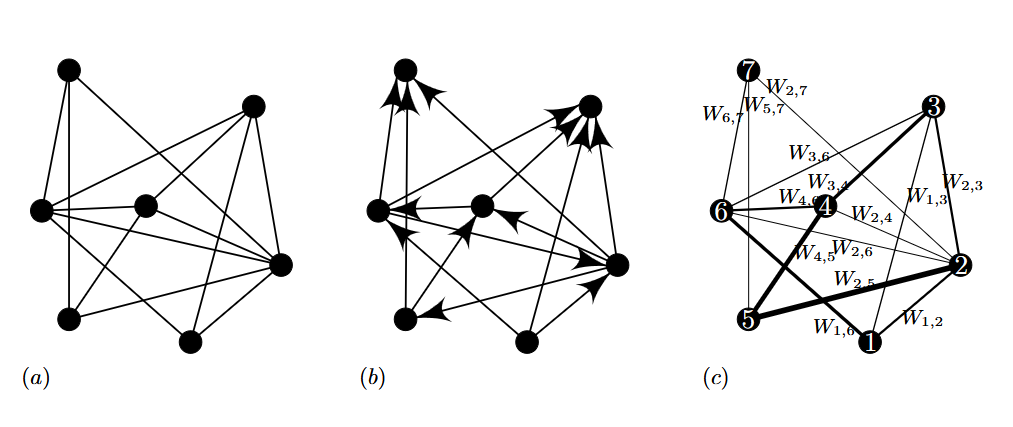
\includegraphics[scale=0.45]{image/weight_graphs.png}
    \caption{Examples of undirected (a), directed (b), weight (c) networks with $N=7$ and $M=12$. The arrows indicates the direction of each link. In the weight graph the thickness of the links represents its weight.}
    \label{fig:weight_graphs}
\end{figure}

\section{Random Networks}
In network theory, random networks play a crucial role in understanding the structure and behavior of complex systems. These networks are often used to model real-world networks, such as the Internet and social networks. There are several methods to generate random networks, each with its own specific focus, such as the degree distribution, the average path length, or the presence of particular structural properties. In this section, we will explore some of the most important models used to generate random networks, highlighting their characteristics and differences.

\subsection{Erd\H{o}s-Rényi Random Graph}

The Erd\H{o}s-Rényi (E-R) random graph $G(N,M)$, where $N$ and $M$ are the number of nodes and links respectively, is one of the first attempts to generate a random network \cite{erdos-renyi1960}. The network is built by randomly choosing $M$ links from all the possible ones. Usually, is used the variation proposed by Gilbert $G(N,p)$ \cite{gilbert} , where $p$ is the probability that two distinct node are connected. The two formulations converge in the thermodynamic limit $N \rightarrow \infty$ and they are interchangeable.
This type of random graph has peculiar properties, such as the degree distribution of the nodes $P(k)$ is binomial
\begin{equation}
    P(k) = \binom{n-1}{k}p^k(1-p)^{n-1-k}
\end{equation} 
Additionally, if $p > \frac{1}{N}$ then is almost sure that the network presents a giant component.
In this work we use the second approach. Figure \ref{E-R_example} shows two examples of E-R random graph, one below and one above the giant component threshold.

\begin{figure}[ht!]
    \centering
    \begin{subfigure}[t]{0.49\textwidth}
        \centering
        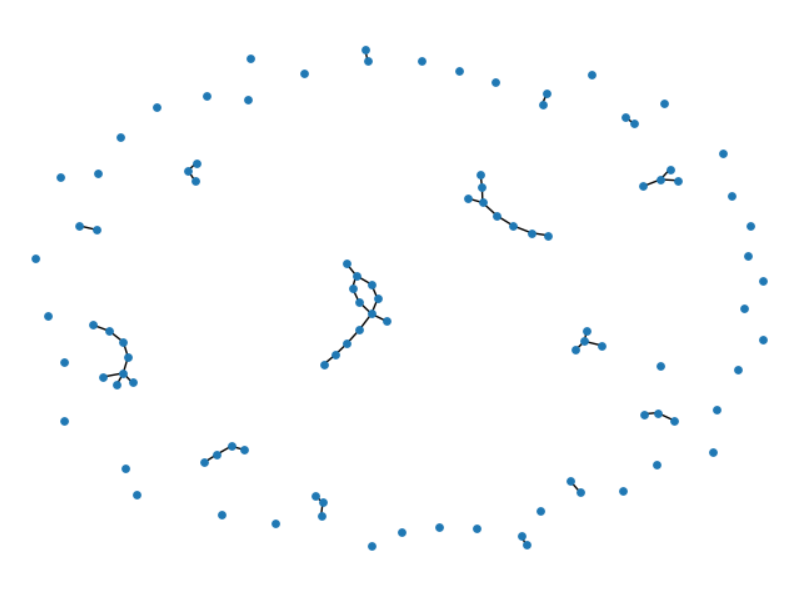
\includegraphics[width=\linewidth]{image/E_R_N100_p0,01.png}
    \end{subfigure}
    \hfill
    \begin{subfigure}[t]{0.49\textwidth}
        \centering
        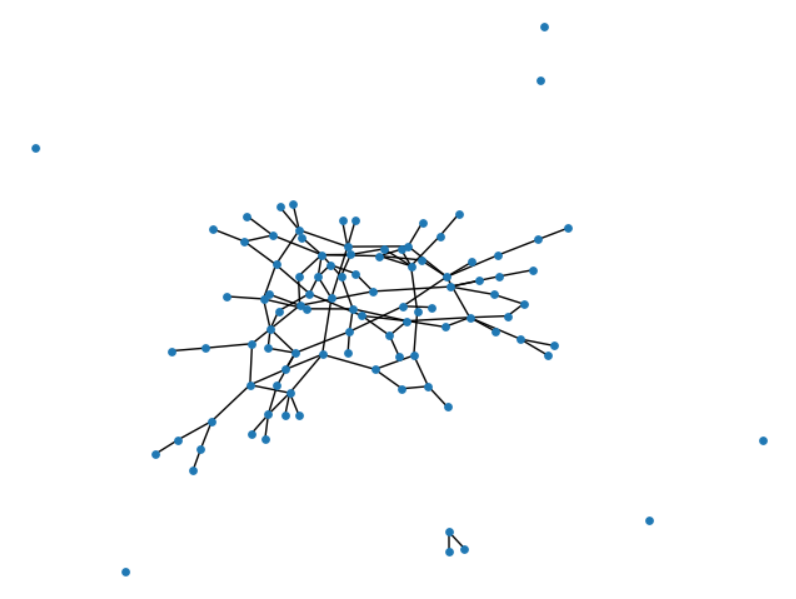
\includegraphics[width=\linewidth]{image/E_R_N100_p0,02.png}
    \end{subfigure}
    \caption{Two examples of Erd\H{o}s-Rényi random graphs: on the left, it has 100 nodes and $p = 0.01$; on the right, it has 100 nodes and $p = 0.02$. Overcoming the threshold $p > 0.01$ can be seen the formation of the giant component.}
    \label{E-R_example}
\end{figure}
%the algorithm is define as below :
%\begin{enumerate}
 %   \item we identify the graph by its adjacency matrix;
 %   \item For each possible link, we generate a random number, if it is less than $p$ the respective entry in the adjacency matrix  is 1 otherwise 0.
%\end{enumerate}

However, the E-R algorithm does not produce networks similar to those found in nature which tend to be more clustered and to have hubs (nodes with very high degree). To simulate these properties, new algorithms have been proposed like the Barab\'abi-Albert scale-free network and the Watts-Strogatz small-world network.

\subsection{Barab\'abi-Albert Scale-Free Network}
Barab\'abi and Albert (B-A) proposed a scale-free network $G(N, m)$, where $N$ is the number of nodes and $m$ is a parameter, that mimics the behavior of real graph like the Internet \cite{Barabasi_Albert_1999}. This type of graph exhibits some preferential nodes which have a degree order of magnitude higher than the average and it presents a power law as degree distribution.
The model works by preferential attachment, where new nodes are more likely to connect to nodes that already have a higher degree. 

The algorithm is defined as follow:
\begin{enumerate}
    \item It is initialized a complete graph of $m_0 > m$ node, usually $m_0 = m+1$;
    \item The other nodes are connected to this graph: for each new node, it is connected to $m$ nodes with probability $p_i = \frac{k_i}{\sum_i k_i}$, where $k_i$ is the degree of the $i$ node.
\end{enumerate}
Figure \ref{B-A_example} shows two examples of B-A networks.

\begin{figure}[ht!]
    \centering
    \begin{subfigure}[t]{0.49\textwidth}
        \centering
        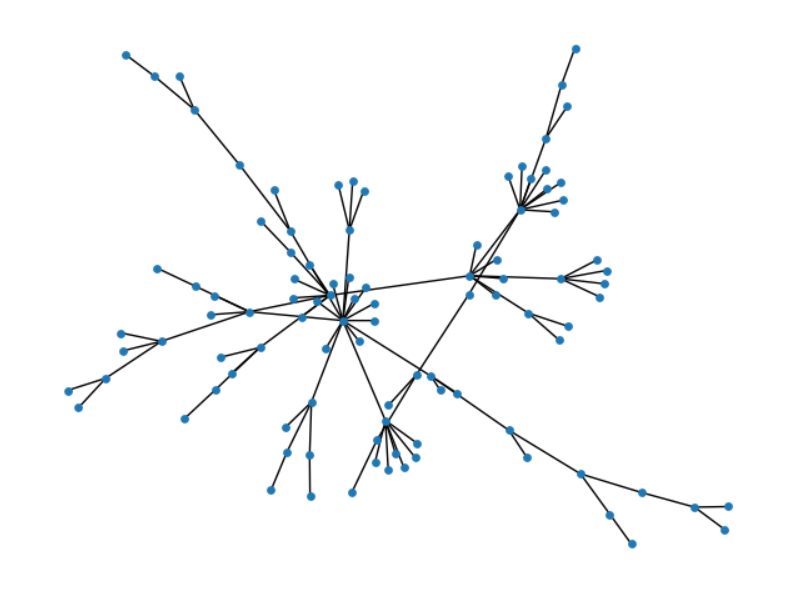
\includegraphics[width=\linewidth]{image/B_A_N100_m1.png}
    \end{subfigure}
    \hfill
    \begin{subfigure}[t]{0.49\textwidth}
        \centering
        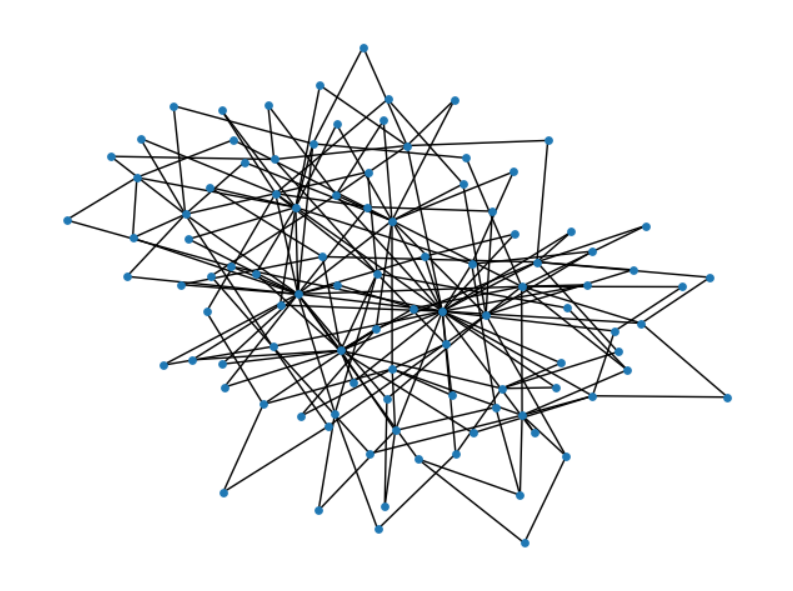
\includegraphics[width=\linewidth]{image/B_A_N100_m2.png}
    \end{subfigure}
    \caption{Two example of Barab\'abi-Albert scale-free networks: on the left, it has 100 nodes and $m=1$; on the right, it has 100 nodes and $m=2$.}
    \label{B-A_example}
\end{figure}

\subsection{Watts-Strogatz Small World Network}

The Watts-Strogatz small-world network $G(N, K, p)$, where $N$ is the number of nodes, $K$ is the average degree (it must be even) and $p$ is the rewiring probability, is a model that exhibits high clustering and short average path lengths \cite{Watts-Strogatz_1998}. The degree distribution follows a power law and the network is homogeneous, meaning that all nodes have similar degree.

The algorithm is defined as follows:
\begin{enumerate}
    \item A ring network with $N$ nodes is created, where each node is connected to the $K/2$ nearest neighbors on each side;
    \item For each edge, with probability $p$ the link is removed and a new one is created to random node. There is no preferential attachments. The new link must be a not existing one.
\end{enumerate}

Figure \ref{W-S_example} it shows two example of W-S networks.

\begin{figure}[ht!]
    \centering
    \begin{subfigure}[t]{0.49\textwidth}
        \centering
        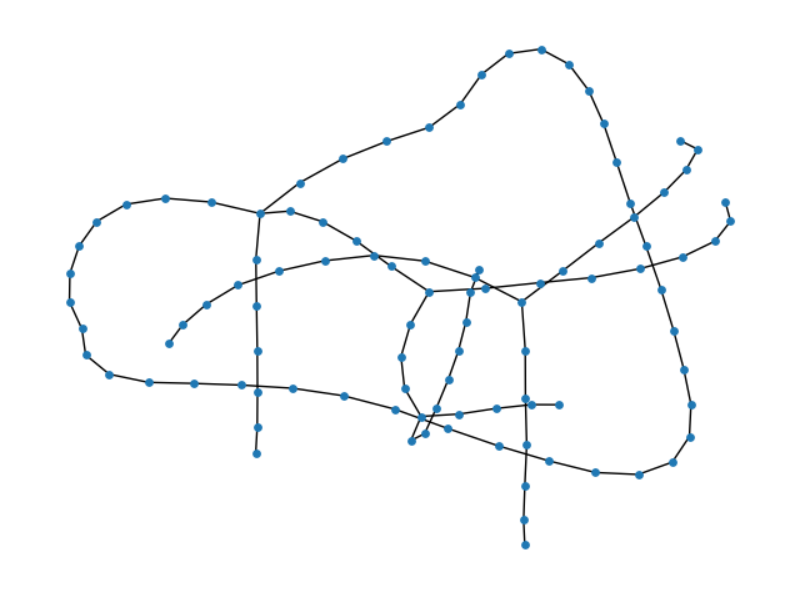
\includegraphics[width=\linewidth]{image/W_S_N100_K2_p0,1.png}
    \end{subfigure}
    \hfill
    \begin{subfigure}[t]{0.49\textwidth}
        \centering
        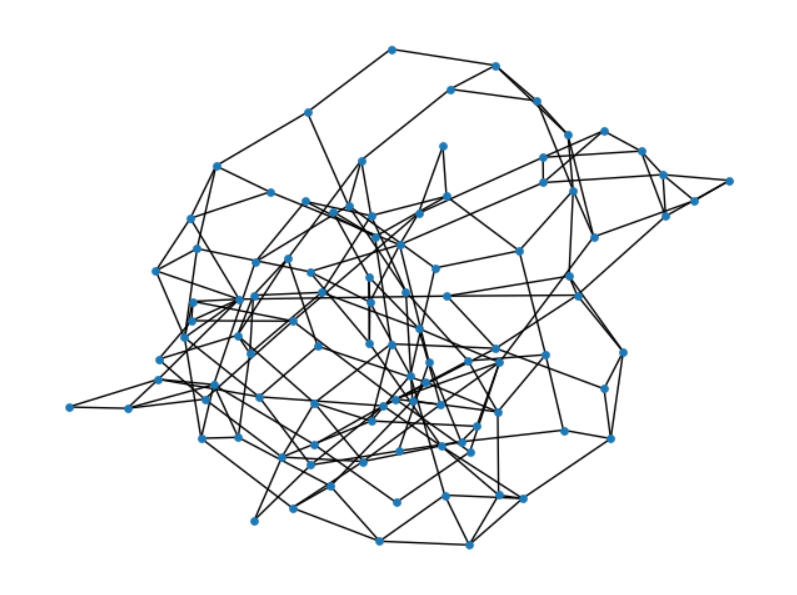
\includegraphics[width=\linewidth]{image/W_S_N100_K4_p0,3.png}
    \end{subfigure}
    \caption{Two example of Watts-Strogatz small world networks: on the left, it has 100 nodes, $K=2$ and $p=0.1$; on the right, it has 100 nodes, $K=4$ and $p=0.3$.}
    \label{W-S_example}
\end{figure}

The B-A and W-S algorithms produce more realistic networks compared to the E-R one, but both focus on their specific feature: the B-A networks fail to reproduce the high clustering of real networks and the W-S ones fail to reproduce the hubs characteristic of networks like Internet.

\section{Random Walk on Networks}

The study of random walks on networks is fundamental in understanding various dynamical processes, such as diffusion, search algorithms, and transport phenomena. In this section, we formalize the mathematical framework of random walks on networks and explore their key properties, including stationary distributions, transition probabilities, and their connection to the Laplacian matrix.

Consider a network $G(N,M)$ where a particle moves randomly between the nodes at each time step, with transition probability $P_{ij}$ to go to the node $j$ starting from the node $i$. If the link between them does not exist then $P_{ij}= 0$. 
The dynamics of this system behaves as a Markov chain: it has no memory of the past states and the future state depends only on the current position.
Let $\rho_i(n)$ be the probability of finding the particle at the node $i$ at time step $n$. The discrete time evolution of the system is given by the law
\begin{equation}
    \rho_i(n+1) = \sum_j P_{ij}\rho_j(n).
\end{equation}

In order to conserve the total probability the transition probability must be a stochastic matrix, namely it must hold 
\begin{equation}
    \sum_i P_{ij}(\Delta t) = 1 .
\end{equation}

The transition probability can be identified with the adjacency matrix of the network
\begin{equation}
    P_{ij} = \frac{A_{ij}}{\sum_j A_{ij}}.
\end{equation}

If the system holds the detailed balance condition
\begin{equation}\label{detail_condition}
    \pi_{ij} \rho_j^* = \pi_{ji} \rho_i^*
\end{equation}
the system admits a unique stationary solution $\rho^*$ such that
\begin{equation}
    \sum_j P_{ij}\rho^*_j =  \rho^*_i .
\end{equation}
This can be written in matrix formalism, where $\Pi$ is the matrix of the transition probability and $\rho^*(t)$ is the stationary probability vector, as
\begin{equation}
    \Pi \rho^* = \rho^*.
\end{equation}
Tus, the stationary distribution is the eigenvector corresponding to the eigenvalue $1$ of the transition matrix.


Taking the continuum limit, we obtain the master equation \cite{Classic_random_walk}
\begin{equation}\label{master_eq}
    \dot \rho_i(t) = \sum_j \pi_{ij}\rho_j(t) - \pi_{ji}\rho_i(t) = - \sum_j L_{ij} \rho_j(t),
\end{equation}
where $\pi_{ij}$ is the transition rate, namely the transition probability per units of time, and $L_{ij} = \sum_k \pi_{kj}\delta_{ij} -\pi_{ij} $ is the Laplacian matrix.
The first term represents incoming transitions to node $i$, while the second term accounts for outgoing transitions.

The Laplacian matrix has the property that $L_{ij} < 0 $ for $i \neq j$ and also it satisfies the relation
\begin{equation}
    \sum_i L_{ij} = 0 .
\end{equation} 

The eigenvalues of the Laplacian matrix have always a not negative real part and its spectrum contains at least one zero eigenvalue, therefore it is not invertible \cite{Boccaletti}. The multiplicity of the zero eigenvalue is equal to the number of connected component of the network: in fact that if the network is not connected the Laplacian should be a block matrix,  block for each connected component, each component can be seen as an independent network with their zero eigenvalue.

The solution of master equation \eqref{master_eq} is
\begin{equation}\label{random_walk_solution}
    \rho(t) = e^{-tL}\rho(0).
\end{equation}

The master equation, in the matrix formalism, for the stationary distribution reduces to 
\begin{equation}\label{stationary_distribution}
    \dot \rho^*(t) = -L \rho^*(t) = 0 . 
\end{equation}
Thus, the stationary distribution is the eigenvector with eigenvalue $0$ of the Laplacian matrix. 
%The other eigenvalues are connected to the Ljapunov exponent and to the time that the occurs to converge to $\rho^*$.

We can prove that
\begin{equation}
    \sum_i \dot\rho_i(t) = - \sum_i \sum_j L_{ij} \rho_j(t) = - \sum_j \left(\sum_i L_{ij}\right) \rho_j(t) = 0 .
\end{equation}
This implies a first integral of motion 
\begin{equation}
    \sum_i \rho_i(t) = \sum_i \rho_i(0) .
\end{equation}

%%add the part with the measure of the eigenvalue, i.e. sum_{\lamda \neq 0} v_\lambda(t) = 0

Let us now assume the network satisfies the detailed balance condition \eqref{detail_condition}, then there exists a hyperplane $\Sigma_0$ that is orthogonal to the stationary distribution and this subspace is invariant under the dynamics. Let be $w \in \Sigma_0$, this subspace is identify by the relation
\begin{equation}
    \sum_i w_i = 0 
\end{equation}
As a matter of fact, let $w(t) \in \Sigma_0$ then 
\begin{equation}
    \sum_i w_i(t+1) = \sum_{ij} \pi_{ij} w_j(t) = \sum_j \underbrace{\left(\sum_i \pi_{ij}\right)}_{1} w_j = \sum_j w_j(t) = 0.
\end{equation}

Therefore, any probability vector can be decomposed as a direct sum of the stationary state and a vector $w(t) \in \Sigma_0$ 
\begin{equation}
    \rho(t) = \rho^* + w(t).
\end{equation}

Furthermore, if the detailed balance condition holds \eqref{detail_condition}, the stationary distribution  is \cite{Classic_random_walk}
\begin{equation}
    \rho^* = \frac{1}{N} \left(1,1,\cdots,1,1\right).
\end{equation} 

The uncertainty in the particle's location can be captured by the Shannon entropy
\begin{equation}
    S = -\sum_i p_i\ln p_i.
\end{equation}
It is a bounded function $0\geq S \geq \ln N$.
It can been shown that the stationary distribution maximizes the Shannon entropy $S = \ln N$.
    
\begin{comment}
    In figure \ref{fig:node_0} is shown only the probability to be in the initial node as a function of time starting  from a Dirac delta distribution for different types of networks\footnote{The python scripts can be found in the GitHub page of the author at the link: \url{https://github.com/ShqemzaMatteo/Master_thesis}}: a ring graph, an Erd\H{o}s-Rényi (E-R) random graph\cite{erdos-renyi1960}, a Barab\'asi-Albert (B-A) scale-free graph\cite{Barabasi_Albert_1999}, and a Watts-Strogatz (W-S) small-sworld graph\cite{Watts-Strogatz_1998}. All the algorithm are explained in the Appendix \Ref{Appendix_A}. 

    \begin{figure}[ht!]
        \centering
        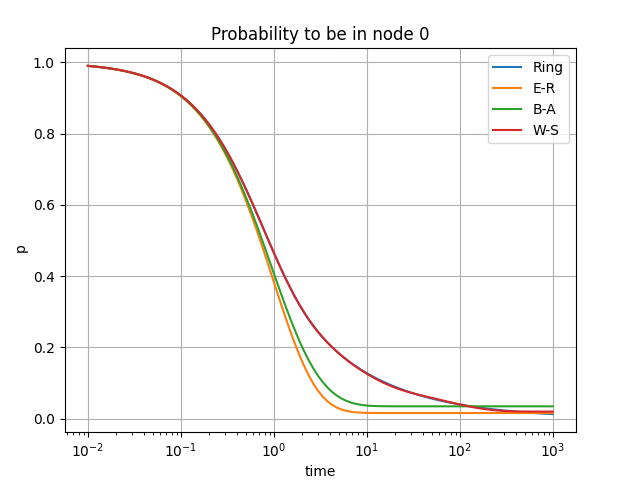
\includegraphics[width=0.65\linewidth]{image/random_graph_node_0.png}
        \caption{Plot of the probability $p$ to be in the node 0 starting from a Dirac delta distribution or the same node as a function of time for different network types of $50$ nodes: a ring graph (blue), a Erd\H{o}s-Rényi (E-R) random graph with connectivity probability $0.7$ (orange), a Barab\'asi-Albert (B-A) scale-free graph with parameter $m=3$ (green), and a Watts-Strogatz (W-S) small world graph with parameter $K=3$ and rewire probability 0.2 (red).}
        \label{fig:node_0}
    \end{figure}
\end{comment}

\section{Quantum Walk}
We can extend the random walk model to quantum particles. 
They must follow the Schrödinger equation with the Laplacian as Hamiltonian. However, the Schrödinger equation requires that the Laplacian is hermitian; therefore, the network must hold the detailed balance condition \eqref{detail_condition}.
This model is known as “continuos time quantum walk" \cite{Farhi_98, quantum_walk}. This model is used to build quantum algorithms \cite{Quantum_walk_Google, classic_to_quantum_networks}.

Let us define an orthonormal basis $\{\ket{i}\}$, where each element $\ket{i}$ indicates their corresponding node $i$, satisfying $\braket{i}{j}=\delta_{ij}$. 
A general general state of the network can be encoded in the ket state $\ket{\psi}$ is define as
\begin{equation}\label{ket_state_quantum}
    \ket{\psi} = \sum_i \sqrt{\rho_i(t)} \ket{i},
\end{equation}
in this way $\rho_i = |\braket{i}{\psi}|^2$ is the projection of the state in the node $i$, in other words the probability that the system can be measured in the node $i$. The norm of $\ket{\psi}$ is normalize to $1$, therefore, the projections $\rho_i$ satisfy the condition $\sum_i \rho_i = 1$.
The Schrödinger equation can be written as
\begin{equation}\label{Schrödinger_quantum_walk}
    \frac{d}{dt}\ket{\psi} = -i\frac{1}{2}\hat L\ket{\psi}.
\end{equation}
where $\hat L = \sum_{ij} L_{ij}\ket{i}\bra{j}$ is the Laplacian operator.
If we apply a Wick rotation into the equation \eqref{Schrödinger_quantum_walk} we recover the master equation of the classic random walk \eqref{master_eq}.

The solution of the equation \eqref{Schrödinger_quantum_walk} takes the form
\begin{equation}
    \ket{\psi(t)} = \hat U(t,0) \ket{\psi(0)} = e^{-\frac{i}{2}\hat L t} \ket{\psi(0)},
\end{equation}
where $\hat U(t,t') =e^{-\frac{i}{2}\hat L (t-t')}$ is the evolution operator and now it is unitary. It holds the following property: $\hat U(t,t')\hat U(t',t'') = U(t,t'')$.

It is possible to define a limiting transition probability for a quantum walk as follow: suppose the system starts at node $\ket{a}$, we measure it after a time $t$, random variable uniformly distributed over the interval $t \in [0,T]$ \cite{quantum_walk}. The transition probability from node $a$ to $b$ is given by
\begin{equation}
    \begin{split}
        \rho_{a\rightarrow b}(T) &= \frac{1}{T}\int_0^T |\bra{a}e^{-i\frac{t}{2}\hat L} \ket{b}|^2 dt\\
        &=\frac{1}{T}\int_0^T \sum_{\lambda,\lambda'}\bra{a}e^{i\frac{t}{2}\hat L}\ket{\lambda}\braket{\lambda}{b} \bra{b}e^{-i\frac{t}{2}\hat L} \ket{\lambda'}\braket{\lambda'}{a} dt\\
        &= \sum_{\lambda,\lambda'}\braket{a}{\lambda}\braket{\lambda}{b}\braket{b}{\lambda'}\braket{\lambda'}{a}\frac{1}{T}\int_0^T e^{-i(\lambda-\lambda')\frac{t}{2}}dt\\
        &= \sum_\lambda|\braket{a}{\lambda}\braket{\lambda}{b}|^2+2\sum_{\lambda\neq\lambda'}\braket{a}{\lambda}\braket{\lambda}{b}\braket{b}{\lambda'}\braket{\lambda'}{a}\frac{1-e^{-i(\lambda-\lambda')\frac{T}{2}}}{i(\lambda-\lambda')T},\\
    \end{split}
\end{equation}
where $\ket{\lambda}$ are the eigenstates of $\hat L$ with eigenvalues $\lambda$. In the limit $T\rightarrow \infty$ it tend to 
\begin{equation}
    \rho_{a\rightarrow b}(T) \xrightarrow[T \rightarrow \infty]{} \sum_\lambda|\braket{a}{\lambda}\braket{\lambda}{b}|^2.
\end{equation}

Let the system be in the state $\ket{\psi}$, also called pure state, we can define the density matrix as
\begin{equation}
    \hat\rho =\ket{\psi}\bra{\psi} = \sum_{ij} \sqrt{\rho_i} \sqrt{\rho_j}\ket{i}\bra{j},
\end{equation}
It is a self-adjoint operator and $\Tr[\hat\rho] = 1$ \cite{Nielsen_Chuang_2010}.

For a generic operator $\hat O(t) = O_{ij}\ket{i}\bra{j}$, the expectation value of the respective observable can be found as
\begin{equation}
        \left< \hat O\right> = \Tr\left[\hat O\hat\rho\right].
\end{equation}
The probability $\rho_k$ to be in the node $k$ can be express using the operator $\hat P_k = \ket{k}\bra{k}$ such that
\begin{equation} \label{state_projection_quantum}
    \begin{split}
        \Tr\left[\hat P_k\hat\rho(t)\right] 
        %= \sum_i \braket{i}{a}\braket{a}{\psi}\braket{\psi}{i}
        %& = \sum_{ijk} \braket{i}{a}\bra{a}\sqrt{\rho_j}\ket{j}\bra{k}\sqrt{\rho_k}\ket{i}\\
        %&= \sum_{ijk} \delta_{i,a}\delta_{a,j}\delta_{k,i}\sqrt{\rho_j}\sqrt{\rho_k}\\
        %= \sqrt{\rho_a}\sqrt{\rho_a} 
        = \rho_k.
    \end{split}
\end{equation}

In the Heisenberg picture, the density operator evolution can be found solving the different equation called Von Neumann equation
\begin{equation}\label{Von Neumann equation}
    \begin{split}
        \frac{d}{dt}\hat\rho(t) 
        %&= \frac{d}{dt}\left(\ket{\psi(t)}\bra{\psi(t)}\right) = \\
        %&= -\frac{i}{2}\hat L\ket{\psi(t)}\bra{\psi(t)} + \ket{\psi(t)}\bra{\psi(t)}\frac{i}{2}\hat L\\
        &= -\frac{i}{2}\left[\hat L,\rho\right]
    \end{split}
\end{equation}
where $[\cdot,\cdot]$ is the commutator.
The solution of the differential equation is
\begin{equation}
    \hat\rho(t) = \hat U(t,0)\hat\rho(0)\hat U^\dagger(t,0) = e^{-\frac{i}{2}t\hat L}\hat\rho\, e^{\frac{i}{2}t\hat L}.
\end{equation}

Using the cyclic property of the trace and the unity of the evolution operator, it can be proved that the $\Tr[\hat\rho]$ is time invariant.

If the initial distribution over the network is uncertain, we can introduce the density matrix for mixed state. Let be $\{\ket{\psi_k}\}_{k<K\in\mathbb{R}}$ a set of different probability state that can describe the system with probability $p_k$, such that $\sum_k^K p_k = 1$, then the mixed density matrix is define as
\begin{equation}
    \hat \rho = \sum_{k=1}^K p_k \hat \rho_k \qquad \hat\rho_k = \ket{\psi_k}\bra{\psi_k}.
\end{equation}

The temporal evolution of the operator is defined as in eq. \eqref{Von Neumann equation}; the probability to be at node a at time t is the same as in eq. \eqref{state_projection_quantum}. All the property for the pure state still holds; this can be easily proven using the linearity of the trace.

Using the mixed density matrix we can consider a system that does not start from a defined distribution, but from an ensemble of possible distribution with their probability. 

To study the mixed state we introduce the Von Neumann entropy
\begin{equation}\label{Von_Neumann_entropy}
    S[\hat\rho]=-\Tr[\hat\rho\ln\hat\rho].
\end{equation}
It is the quantum counterpart of the Shannon entropy for classical information theory.
The Von Neumann entropy \eqref{Von_Neumann_entropy} is bounded $0\geq S[\hat\rho] \geq \ln N$. It vanishes for pure states.
The Von Neumann entropy is a time invariance, thus, the evolution operator takes pure state into pure state \cite{Nielsen_Chuang_2010}.
\begin{comment}
    \begin{equation}
        \begin{split}
            S[\hat\rho(t)] &=\Tr[\hat\rho(t)\ln\hat\rho(t)]= \Tr[U(t,0)\hat\rho(t)U^\dagger(t,0)\ln\left(U(t,0)\hat\rho(t)U^\dagger(t,0)\right)]\\
            &=\Tr[U(t,0)\hat\rho(0)U^\dagger(t,0)U(t,0)\ln\left(\hat\rho(0)\right)U^\dagger(t,0)]\\
            &= S[\hat\rho(0)].
        \end{split}
    \end{equation}
    We can move out the evolution operator because they are unitary, since if we consider the taylor expansion
    \begin{equation}
        \begin{split}
            \ln\left(U(t,0)\hat\rho(t)U^\dagger(t,0)\right) &= c_0U(t,0)U^\dagger(t,0) + c_1 U(t,0)\hat\rho(t)U^\dagger(t,0)\\
            & \quad + c_2 U(t,0)\hat\rho(t)U^\dagger(t,0)U(t,0)\hat\rho(t)U^\dagger(t,0) + ... \\
            &=  U(t,0)\ln\left(\hat\rho(t)\right) U^\dagger(t,0).
        \end{split}
    \end{equation}
\end{comment}

\begin{comment}
If we consider the system in contact with a thermal bath with which exchange only energy but conserving it in average, namely the canonical condition hold, there is a stationary state $\hat\rho = e^{-\beta \hat L}$ that maximize the entropy. The parameter $\beta$ is just the inverse of a pseudo-temperature that stands for the interaction with the thermal bath. 
Since the thermal bath actively changes the entries of $\hat L$, it is changing the weight of the network and the probability to move from node $i$ to $j$. Thus, we are considering a network that is changing randomly by time. 
The reader can recognize that this density matrix is the same the De Domenico has introduced \eqref{density_matrix}.
\end{comment}

\subsection{1-D Quantum Random Walk}
Consider a toy model: the quantum random walk over a discrete line \cite{Farhi_98}. The probability of moving left or right is $\frac{1}{2}$.
To analyze this model, it is useful to introduce the momentum state $\ket{p}$ such that $\braket{j}{p} = e^{ijp}$, where $-\pi < p< \pi$.

In line the Laplacian is defined as
\begin{equation}
    \hat L \ket{j} = 2\ket{j} -\ket{j-1} -\ket{j+1} . 
\end{equation}
Therefore, applying this to the momentum state
\begin{equation}
    \begin{split}
        \bra{j}\hat L \ket{p} &= \braket{j}{p} -\frac{1}{2}\braket{j-1}{p} -\frac{1}2{}\braket{j+1}{p}\\
        &= e^{ijp} -\frac{1}{2}e^{i(j-1)p} - \frac{1}{2}e^{i(j+1)p}\\
        &= e^{ijp}(\cos(p) - 1) = (\cos(p) - 1)\braket{j}{p}
    \end{split}
\end{equation}

Thus, the amplitude of the walk can be computed as the integral over all the momenta, leading to
\begin{equation}
    \begin{split}
        \bra{j}e^{-i\frac{t}{2}\hat L} \ket{k}&= \frac{1}{2\pi}\int_{-\pi}^{\pi} e^{-i\frac{t}{2}(\cos(p) - 1)} \braket{j}{p} \braket{p}{k} dp\\
        &= \frac{1}{2\pi}\int_{-\pi}^{\pi} e^{-ip(j-k)-i\frac{t}{2}(\cos(p) - 1)}\\
        & = e^{i\frac{t}{2}}(-i)^{k-j}J_{k-j}\left(\frac{t}{2}\right),
   \end{split}
\end{equation}
where $J_{n}(x)$ is the Bessel function of the first kind of order $n$.

Applying the Wick rotation we obtain 
\begin{equation}\label{Bessel_function}
    \left|\bra{j}e^{-i\frac{t}{2}\hat L} \ket{k}\right|^2 = e^{-t} \left(I_{k-j}\left(\frac{t}{2}\right)\right)^2,
\end{equation}
where $I_{n}(x) = i^{n}J_{n}(ix)$ is the modified Bessel function of the first kind.
In the limit $t\gg 1$ it tends to a gaussian centered in the origin and variance $\sqrt{t}$, in accordance with the classical model \cite{mabramowitz64:handbook}.

\subsection{Double tree network}
Another important toy model is the quantum walk on a network consisting of two binary trees of depth $n$ with the ending connected as shown in figure \ref{fig:Double_Tree}.
We start from one root and analyze the probability to reach the other one \cite{quantum_walk}.
Classically, the probability of crossing the network scales exponentially as $2^{-n}$, and it is not computable for big $n$.
However, using the quantum version it remains computable.
\begin{figure}[ht!]
    \centering
    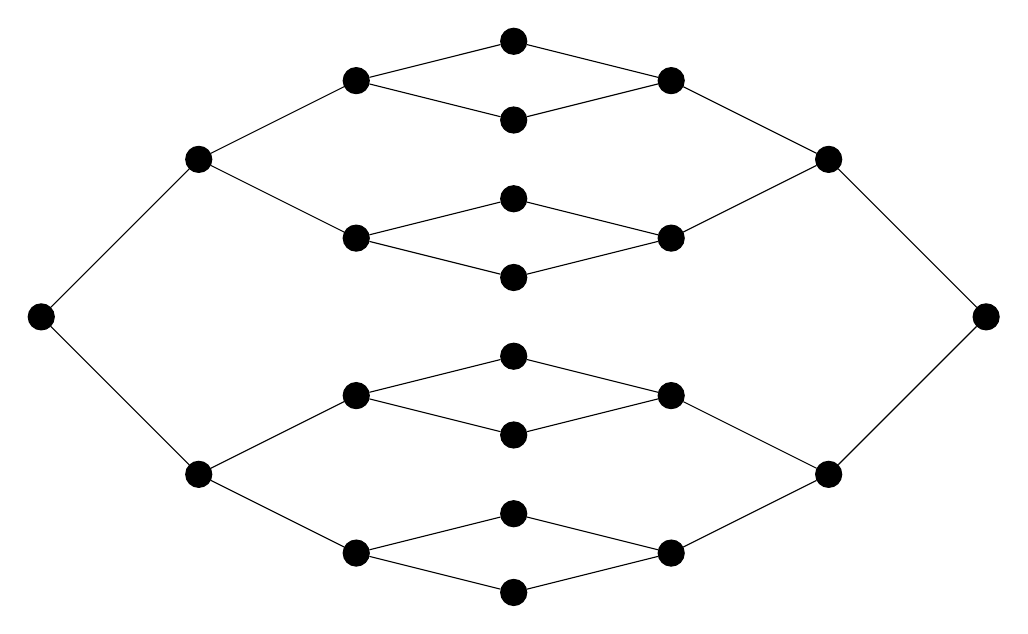
\begin{tikzpicture}[>=stealth, node distance=2cm, every node/.style={circle, draw, fill=black}]
        %draw nodes by coordinates
        \node (n00) at (-6,0) {};
        \node (n11) at (-4,2) {};
        \node (n12) at (-4,-2) {};
        \node (n21) at (-2,3) {};
        \node (n22) at (-2,1) {};
        \node (n23) at (-2,-1) {};
        \node (n24) at (-2,-3) {};
        \node (n31) at (0,3.5) {};
        \node (n32) at (0,2.5) {};
        \node (n33) at (0,1.5) {};
        \node (n34) at (0,0.5) {};
        \node (n35) at (0,-0.5) {};
        \node (n36) at (0,-1.5) {};
        \node (n37) at (0,-2.5) {};
        \node (n38) at (0,-3.5) {};
        \node (n41) at (2,3) {};
        \node (n42) at (2,1) {};
        \node (n43) at (2,-1) {};
        \node (n44) at (2,-3) {};
        \node (n51) at (4,2) {};
        \node (n52) at (4,-2) {};
        \node (n60) at (6,0) {};
        
        % Draw edges (links)
        \draw (n00) -- (n11);
        \draw (n00) -- (n12);
        \draw (n11) -- (n21);
        \draw (n11) -- (n22);
        \draw (n12) -- (n23);
        \draw (n12) -- (n24);
        \draw (n21) -- (n31);
        \draw (n21) -- (n32);
        \draw (n22) -- (n33);
        \draw (n22) -- (n34);
        \draw (n23) -- (n35);
        \draw (n23) -- (n36);
        \draw (n24) -- (n37);
        \draw (n24) -- (n38);
        \draw (n31) -- (n41);
        \draw (n32) -- (n41);
        \draw (n33) -- (n42);
        \draw (n34) -- (n42);
        \draw (n35) -- (n43);
        \draw (n36) -- (n43);
        \draw (n37) -- (n44);
        \draw (n38) -- (n44);
        \draw (n41) -- (n51);
        \draw (n42) -- (n51);
        \draw (n43) -- (n52);
        \draw (n44) -- (n52);
        \draw (n51) -- (n60);
        \draw (n52) -- (n60);
    \end{tikzpicture}
    \caption{The picture of a glued double tree network.}
    \label{fig:Double_Tree}
\end{figure}

To simplify the analysis, we can introduce a new basis $\ket{\mathrm{col}\; j}_{j<2n}$ that indicates a column and not the single node, except at the two root nodes where they coincide. This basis is defined as
\begin{equation}
    \ket{\mathrm{col}\; j} = \frac{1}{\sqrt{N_j}}\sum_{a\in \mathrm{column}} \ket{a}, 
\end{equation}
where the renormalization factor $N_j$ is 
\begin{equation}
    N_j = \left\{\begin{aligned}
        &2^j \qquad &0\leq j\leq n\\
        &2^{2n-j} \qquad &n \leq j \leq 2n
    \end{aligned}\right. .
\end{equation}

In this basis, the Laplacian act as
\begin{equation}
    \begin{aligned}
        \bra{\mathrm{col}\; j}\hat L \ket{\mathrm{col}\; j} &= 1\\
        \bra{\mathrm{col}\; j \pm 1}\hat L \ket{\mathrm{col}\; j} &=\left\{\begin{aligned}
            \frac{\sqrt{2}}{2} \qquad j=0,n,2,\\
            \frac{\sqrt{2}}{3} \qquad \mathrm{otherwise}\\
        \end{aligned}\right.
    \end{aligned}
\end{equation}

Thus, the dynamics along the network reduces to a 1-D quantum walk which has a known computable solution \eqref{Bessel_function} %\cite{quantum_walk}
\begin{equation}
    \bra{0}e^{i\frac{t}{2}\hat L}\ket{2n} = e^{-t} I_{2n}\left(\frac{t}{2}\right),
\end{equation}
where $I_{n}(x) = i^{n}J_{n}(ix)$ is the modified Bessel function of the first kind. 


\chapter{Density Matrix and Entropy for Networks}\label{C_Density_Matrix}

In many complex systems, one element can be influenced by others with which does not directly interact. For instance, considering the city mobility, the road forms a network, closing one road may create traffic in other roads that do not intersect the closed one. To study the correlations between the nodes of a network the communicability matrix was introduced \cite{Estrada_2008}. 
This matrix captures the way the information spreads across the network. Thus, it should depend on the dynamical aspects of the network.
We call it communicability because correlation as a different meaning in social science, where it typically describes interactions.

Interestingly, this matrix behave as quantum density matrix, making it is a possible candidate to the role of network's density matrix. As a consequence, we can introduce an entropy function analogous to the Von Neumann entropy found in quantum many body and quantum computing, opening a connection between the network theory and quantum realm.

\section{Estrada's Communicability matrix}

Most of the study on complex networks focuses on the spread of information following the shorter path, namely the shortest sequence of links that connects two different nodes. 
However, this is not the only way the information can flow, there are plenty of other more long route that are also available, and this vision ignores completely the complexity of the network.
To overcome that we introduce the communicability matrix, defined to consider also these possible path to go beyond the shortest one \cite{Estrada_2012}. It consider the influence over all the path that cross the choose node, weighted by their length.
%This concept is similar to the correlation in physics: it indicates how a node is changes in response to a perturbation in another node. 

Let $G=(V,E)$ be an undirected graph composed of $N$ nodes and $E$ links and let $A$ be the adjacency matrix of the graph.
We can define the communicability matrix as
\begin{equation}
    G(A) = \sum_{k=1}^{\infty}c_k A^k
\end{equation}
and the communicability from node $i$ to node $j$ is given by $G_{ij}$. The power of the adjacency matrix $(A^k)_{ij}$ give us the number of path of length $k$ starting from node $i$ ending in node $j$.
The coefficients $c_k$ indicates the weight of the paths and it is heavier the longer is the path, this is made to give more relevance to the short ones respect to the long ones. It must be chosen such that the series is convergent, they also must penalize long paths to reflect the preference to the shorter one.

An intuitive choice is $c_k = \frac{1}{k!}$, which transforms the communicability into an exponential function \cite{Estrada_2008}
\begin{equation}\label{G_E}
    G^E(A) =\sum_{k=1}^{\infty} \frac{A^k}{k!} = e^{A} .
\end{equation}
We can generalize it adding a constant term $\beta$
\begin{equation}
    G^E(A) =\sum_{k=1}^{\infty} \frac{\beta A^k}{k!} = e^{\beta A} ,
\end{equation}
this formulation is similar to the thermal green function for quantum system with Hamiltonian $A$ and temperature $T = \frac{1}{\beta}$.

Alternatively, we can choose $c_k = \alpha^{k}$ with $\alpha<\frac{1}{\lambda_N}$, where $\lambda_N$ is the largest eigenvalue of the adjacency matrix \cite{Katz}. In this case, it becomes a geometrical series yielding
\begin{equation}\label{G_R}
    G^R(A) =\sum_{k=1}^{\infty} \alpha^k A^k = (I -\alpha A)^{-1}.
\end{equation}
The two formulations for the communicability matrix lead to the same result and conclusion for the network in the limit $\alpha \rightarrow \frac{1}{\lambda_N}$ and $\lambda_N -\lambda_{N-1}$ large \cite{Benzi_Klymko}.


From this, we can introduce an global index for the network that consider all the different possible communication as
\begin{equation}
    EE(A)  = \Tr\left[e^{\beta A}\right].
\end{equation}
In the literature it is called Estrada index \cite{Estrada_2008} and can be interpreted as the sum of all the self-communication, that is the sum of the paths that end in the same node they have started.

However, the communicability matrices \eqref{G_E} and \eqref{G_R} study only the network's topology, namely the paths, and ignore the presence of dynamics over the network that may change the way information spreads.

If we consider the simplest dynamics, the random walk, it is governed by the Laplacian matrix $L$. 
Thus, the communicability matrices for random walk are \cite{Estrada_2012}
\begin{equation}\label{Estrada indeces}
    \begin{split}
        G^E(L) &=\sum_{k=1}^{\infty} \frac{\beta^k L^k}{k!} = e^{\beta L}  \\ 
        G^R(L) &= \sum_{k=1}^{\infty} \alpha^k L^k \rightarrow \alpha^{-1} \tilde{L}^{-1}
    \end{split}
\end{equation}

where $\tilde{L}^{-1} = \sum_{i=2}^N \frac{1}{\mu}v_i^Tv_i$ is the Moore-Penrose generalized inverse of the Laplacian. Here, $\mu$ are the eigenvalue ordered from the smaller to the bigger such that $\mu_1 < \mu_2 < ... < \mu_N$, and $v_i$ the respective eigenvectors of the Laplacian matrix \cite{Generalized_inverse_Laplacian}.
Also, the Laplacian Estrada index is define as
\begin{equation}\label{EE_L}
    EE(L) = \Tr\left[e^{\beta L}\right].
\end{equation}

%While the previous quantities using the adjacency matrix focalized over the topological aspects of the network and information spread, the laplacian communicability matrix embodies also the dynamical ones since the laplacian is involved in the random walk over a network. 

\subsection{Hamiltonian formalism}
The formulae \eqref{Estrada indeces} can be motivated by studying a classic and quantum harmonic oscillator on a network.
Consider a set of $N$ harmonic oscillators with coupling matrix $K = A$, where $A$ is a symmetric adjacency matrix. In this way, the nodes are considered as particle of mass $m = 1$ connected by springs with constant $A_{ij}$. The network should not have self interacting nodes, thus $A_{ii} = 0$. The system is submerged in a thermal bath at the temperature $T$. We assume there are no dumping and no external forces acting in the system besides the thermal fluctuation. 
Let introduce a set of coordinates $q_i$ that indicates the displacement of the $i$ particle respect the equilibrium position, the elastic elastic potential can be define as
\begin{equation}
    V(q) = \frac{1}{4}\sum_{i\neq j} K_{ij}(q_i-q_j)^2 = \frac{1}{2}\sum_{j}K_{jj}q_j^2 - \frac{1}{2} \sum_{i\neq j}K_{ij}q_iq_j,
\end{equation}
where 
\begin{equation}
    K_{jj} = \sum_{j \neq i} K_{ij}.
\end{equation}

We set $H_{ij}= K_{jj}\delta_{ij} - K_{ij}$, therefore the potential can be written as
\begin{equation}
    V(q) = \frac{1}{2}\sum_{i,j} H_{ij} q_i q_j.
\end{equation}
The $H$ matrix is a laplacian matrix and it is equal to the Laplacian of the network $L = D - A$, where $D$ is the degree matrix. It holds the property $\sum_j H_{ij} = 0$, therefore it has not negative eigenvalues and one must be equal to zero.
The zero eigenvalue ensure us that the motion of the center of must is conserved. %% find a way to cite this sentence

We can write the Lagrangian of the system as
\begin{equation}
    \mathcal{L} = \frac{1}{2}\sum_{ij} \dot q_i G_{ij} \dot q_j - \frac{1}{2} \sum_{ij} q_iH_{ij}q_j.
\end{equation}

The equations of motion are
\begin{equation}
    \ddot q_i = -H_{ij} q_j.
\end{equation}

The eigenmodes of the system are defined by the solution of the equation 
\begin{equation}
    \omega^2 \phi_i = H_{ij} \phi_j.
\end{equation}

Rewriting it in matrices form
\begin{equation}
    |\Omega^2 - H| = |\Omega^2 - H|.
\end{equation}

Therefore, the spectral signature of the matrix $H = L$ are the same of the harmonic oscillator. In this way we can connect the harmonic oscillator and the master equation of a network and vice versa. Since $M$ is diagonal, $H$ and $L$ have the same support, eigenvectors and eigenvalues, leading to $E = \omega^2 = \lambda$, which creates a natural ranking between the eigenvectors. 

The Hamiltonian of the system is given by
\begin{equation}\label{H_L}
    H_L = \sum_i \frac{p_i^2}{2} + \sum_{ij} \frac{1}{2}L_{ij}q_iq_j.
\end{equation}

\subsection{Network of classic harmonic oscillators}

To combine this with the thermodynamics, let consider the presence of a thermal bath in the Hamiltonian formalism using the Langevin equation
\begin{equation}
    \begin{aligned}
        &\dot q_i = p_i; \\
        &\dot p_i  = -H_{ij}q_j - \gamma \sum_j \left(\delta_{ij} - 1_{ij}\right)p_j + \sqrt{2T\gamma}\xi_i(t),
    \end{aligned}
\end{equation}
where $\gamma$ is the friction coefficient, $T$ is the temperature (Boltzmann constant $K_B =1$), $\delta_{ij}$ the Kronecker delta and $1_{ij}$ the matrix with all entries equal to 1, $\xi_i(t)$ is white noise, namely
\begin{equation}\label{white_noise}
    \langle\xi_i(t)\rangle = 0 \qquad \langle\xi_i^2(t)\rangle = 1 
\end{equation}

The white noises must hold the condition $\sum_i \xi_i = 0$, that leaves invariant the motion of  system's center of mass but $\xi_i(t)$ are no more independent.
As a matter of fact, the derivative of $\sum_i p_i$ is zero, therefore it is an integral of motion,
\begin{equation}
    \frac{d}{dt} \sum_i \dot p_i = - \gamma \sum_{ij}\left(\delta_{ij} - 1_{ij}\right)p_j+ \cancel{\sqrt{2T\gamma}\sum_i\xi_i(t)} = 0.
\end{equation}

The condition over the white noises $\sum_i \xi_i = 0$ adds breaks the independence between them and it adds correlation.
We can rewriting the noise using i.i.d. white noise $w_i(t)$ as
\begin{equation}
    \xi_i(t) = w_i (t) + \frac{1}{N} \sum_k w_k(t).
\end{equation}
The covariance matrix of $\xi_i(t)$ can be written as
\begin{equation}
    \left<\xi_i(t)\xi_j(s)\right> = \left[\delta_{ij} - 1_{ij}\right]\delta(t-s)
\end{equation}

The distribution $\rho(q,p,t)$ is a Gaussian and satisfies the Fokker-Plank equation \cite{Fokker}
\begin{equation}
    \frac{\partial\rho}{\partial t} = -\sum_i p_i\frac{\partial \rho}{\partial q_i} + \sum_{ij} H_{ij}q_j\frac{\partial \rho}{\partial p_i} + \gamma\sum_{ij}\left(\delta_{ij}-1_{ij}\right)\left[\frac{\partial}{\partial p_i}p_j\rho + T \frac{\partial^2\rho}{\partial p_i \partial p_j}\right].
\end{equation}
The dynamics converges to a stationary distribution with time scale depending on the eigenvalue of the Laplacian matrix.  
The solution at equilibrium is
\begin{equation}
    \rho(q,p) = Z(\beta)^{-1} \exp\left[ -\beta \left( \sum_j {p_j^2} + \sum_{ij} \frac{1}{2}q_iH_{ij}q_j\right)\right],
\end{equation}
where $\beta = \frac{1}{T}$ and $Z(\beta)$ is the partition function defined as
\begin{equation}
    Z(\beta) = \int \prod_i dp_i dq_i \; \exp\left[ -\beta \left( \sum_j {p_j^2} + \sum_{ij} q_iH_{ij}q_j\right)\right].
\end{equation}

The marginal distribution on the coordinates is a Maxwell-Boltzmann distribution with the internal energy 
\begin{equation}
    \rho(q) = Z(\beta)^{-1} e^{-\beta \left(\sum_{ij} q_iH_{ij}q_j\right)}.
\end{equation}

If $H$ is symmetric, namely the detailed balance condition holds, we can diagonalize the equation obtaining the motion of independent oscillators in the same thermal bath.
Therefore, changing the basis from $q_i$ to $Q_\lambda$ eigenvectors of the Hamiltonian, the marginal distribution becomes
\begin{equation}\label{marginal_probability}
    \rho(q) = Z(\beta)^{-1} e^{-\beta \left(\sum_{\lambda \neq 0} Q_\lambda \lambda Q_\lambda\right)},
\end{equation}
with partition function 
\begin{equation}
    Z(\beta) = \int \prod_{\lambda\neq 0} dQ_\lambda e^{-\beta \left(\sum_{\lambda \neq 0} \lambda Q_\lambda^2\right)}.
\end{equation}

The thermal distribution does not involve the zero eigenmode since the thermal bath does not interact with it. Thus, we can project the system into a invariant subspace orthogonal to the stationary distribution. The oscillator modes $Q_\lambda$ remain the same of the unperturbed case. 
This is a consequence of the condition $\sum_i \xi_i = 0$.
%Moreover, this is also connected to the conservation of the stationary distribution of the master equation \eqref{stationary_distribution}. 
The distribution has mean $\left<Q_\lambda\right>= 0$ and the covariance matrix is diagonal with entries $\left<Q^2_\lambda\right>= \frac{1}{\beta \lambda}$.

The variance can be expresses as
\begin{equation}\label{classic_correlation}
    \mathrm{Cov}(Q) = \frac{1}{\beta}L^{-1},
\end{equation}
where ${L}^{-1} = \sum_{i=2}^N \frac{1}{\mu_i}v_i^Tv_i$ is the Moore-Penrose generalized inverse of the Laplacian. Here, $\mu$ are the eigenvalue ordered from the smaller to the bigger such that $\mu_1 < \mu_2 < ... < \mu_N$, and $v_i$ the respective eigenvectors of the Laplacian matrix \cite{Generalized_inverse_Laplacian}.

This is the same result as the Estrada's Communicability matrix $G^R(L)$ \eqref{Estrada indeces} with $\alpha=\beta$.
When $T\rightarrow 0$ the spread of information drops; and when $T\rightarrow +\infty$ it becomes instantaneous.

\subsection{Network of quantum harmonic oscillators}

Instead, for the quantum case ($\hbar = 1$), $H_L$, $q_i$ and $p_j$ are promoted to operators $\hat H_L$, $\hat q_i$ and $\hat p_j$ and  they satisfy the commutator relation $\left[\hat q_i, \hat p_j\right] = i \delta_{ij}$.

We need to add a new term; it should be considered as additional springs with constant $K'$ that connect each node to the ground: it prevent the the center of mass from moving. So the Hamiltonian becomes
\begin{equation}\label{H_L_QM}
    H_L = \sum_i\left(\frac{\hat p_i^2}{2}+\frac{K'}{2}\hat q_i^2\right) + \sum_{ij}\frac{1}{2} L_{ij}\hat q_i\hat q_j.
\end{equation}

We introduce the bosons creation and annihilation operators as
\begin{equation}
     \hat a_i = \frac{1}{\sqrt{2}}\left(\sqrt{\Omega} \hat q_i + \frac{i}{\sqrt{\Omega}}\hat p_i\right) \qquad 
     \hat a_i^\dagger = \frac{1}{\sqrt{2}}\left(\sqrt{\Omega} \hat q_i - \frac{i}{\sqrt{\Omega}}\hat p_i\right), 
\end{equation}
and the inverse as
\begin{equation}
    \hat q_i = \sqrt{\frac{1}{2\Omega}}\left(\hat a_i + \hat a_i^\dagger\right) \qquad
    \hat p_i = i\sqrt{\frac{\Omega}{2}}\left(\hat a_i - \hat a_i^\dagger\right),
\end{equation}
where $\Omega = \sqrt{K'}$.
They satisfy the commutation relation $\left[\hat a_i, \hat a^\dagger_j\right] = \delta_{ij}$. 

The Hamiltonian can be written as 
\begin{equation}
    \hat H_L = \sum_i \Omega \left(\hat a_i\hat a^\dagger_i + \frac{1}{2}\right) + \frac{1}{4\Omega}\sum_{ij}\left(\hat a_i +\hat a_i^\dagger\right)L_{ij}\left(\hat a_i +\hat a_i^\dagger\right).
\end{equation}

Since The network is undirected, $L$ is symmetric and, therefore, we can diagonalize it. The diagonalized laplacian is written in the form $\Lambda = OLO^T$.
This generates a new pair of bosons creation and annihilation operators respect the eigenvalue $\mu$ of the Laplacian
\begin{equation}
    b_\mu = \sum_j a_jO_{\mu j}  \qquad \hat b_\mu^\dagger = \sum_j a_j^\dagger O^T_{\mu j} .
\end{equation}

Thus, the new Hamiltonian becomes a sum of independent Hamiltonians
\begin{equation}
    \hat H_L = \sum_\mu \hat H_\mu,
\end{equation}
with
\begin{equation}
    \begin{split}
        \hat H_\mu &= \Omega \left(\hat b_\mu\hat b^\dagger_\mu + \frac{1}{2}\right) + \frac{1}{4\Omega}\mu\left(\hat b_\mu +\hat b_\mu^\dagger\right)^2\\
        &= \Omega \left(\hat b_\mu\hat b^\dagger_\mu + \frac{1}{2}\right) + \frac{1}{4\Omega}\mu\left[\left(\hat b_\mu\right)^2 +\left(\hat b_\mu^\dagger\right)^2 + 2 \hat b_\mu \hat b_\mu^\dagger + 1 \right]\\
        &= \Omega \left[ 1 + \frac{1}{2\Omega}\mu\right] \left(\hat b_\mu\hat b^\dagger_\mu + \frac{1}{2}\right) + \frac{1}{4\Omega}\mu\left[\left(\hat b_\mu\right)^2 +\left(\hat b_\mu^\dagger\right)^2 \right].
    \end{split}
\end{equation}

We now consider the system as fermionic so the modes do not excite beyond the first excitation state. In this way we can restrict the Hilbert state of a mode to the span of the ground state $\ket{g}$ and the first excited state $\ket{e_\mu}=b_\mu^\dagger\ket{g}$. A consequence of it is that the second term in the Hamiltonian cancel out. 


Now, we can compute the thermal Green function or Matsubara Green function for fermions $G$. This quantity describes the probability amplitude for the particle to travel from one state to the other in a given time $\tau$ (more detail in the Appendix \ref{Appendix_B}). For $\tau > 0$ it is

\begin{equation}
    \begin{split}
        G^L_{ij}(\beta, \tau > 0) &= \frac{\Tr\left[e^{-\beta \hat H_L}\hat a_i (\tau)  \hat a_j^\dagger\right]}{\Tr\left[e^{-\beta \hat H_L}\right]} \\
        &=\sum_{\mu\nu} O_{\mu i}\frac{\Tr\left[ (\tau) e^{-\beta \hat H_L} \hat b_\mu\hat b_\nu^\dagger\right]}{\Tr\left[e^{-\beta \hat H_L}\right]}O_{j\nu}\\
        &= \sum_{\mu} O_{i\mu}\left\{-e^{-\mu \tau}\left[\left(1-f\left( \Omega + \frac{1}{2\Omega^2}\mu\right)\right)\Theta(\tau)\right]\right\}O_{j\mu}\\
        &= \sum_{\mu} O_{i\mu}\left\{\frac{e^{-\mu \tau}}{e^{-\beta\left[ \Omega + \frac{1}{2\Omega^2}\mu\right]} + 1}\right\}O_{j\mu}\\
    \end{split}
\end{equation}
In the limit $\tau \rightarrow 0^+$ and $\beta$ large enough it tend to
\begin{equation}
    G^L(\beta) = \sum_{\mu} O_{i\mu}{e^{\beta\left[ \Omega + \frac{1}{2\Omega^2}\mu\right]}} O_{\mu i},
\end{equation}
that can be written as
\begin{equation}
    G^L_{ij}(\beta)= e^{\beta \Omega}e^{\frac{\beta \omega^2}{2\Omega}L}.
\end{equation}

Comparing it with the eq. \eqref{Estrada indeces}, choosing $2\Omega =\omega^2$ the two equations are related as
\begin{equation}
    G^R(L) = e^{-\beta\Omega}G^L(\beta).
\end{equation}
When the temperature $T \rightarrow 0$ the communicability between the nodes drops to zero and the perturbation does not spread across the network. Instead, when $T \rightarrow \infty$ the communicability tend to infinity and the perturbation spread instantaneously.  


\section{Density matrix and entropy for complex network}
%as in paper 2023 with the special case in paper 2020
The communicability matrix defined above possesses peculiar properties that make it suitable for use as a density matrix. Moreover, the presence of the Laplacian matrix ensure that it does not only consider the topological features of the network but also the dynamics. Taking the exponential communicability matrix as a reference, we can define a density matrix as
\begin{equation}\label{density_matrix}
    \hat \rho(\beta) = \frac{1}{Z} e^{-\beta \hat L} \qquad \mathrm{with} \qquad Z(\beta) = \Tr[e^{-\beta \hat L}],
\end{equation}
where $Z$ is the partition function and it is equal to the Laplacian Estrada index of the network \eqref{EE_L}.
It is a hermitian and positive defined matrix with trace equal to unity. 
It can be seen that $e^{-\beta L}$ is the propagator for diffusion equation in a network at time $t = \beta$.

From this, we can define the network's entropy as the Von Neumann entropy
\begin{equation} \label{entropy}
    S(\hat\rho) = -\Tr[\hat \rho \ln \hat \rho].
\end{equation}

Considering \eqref{density_matrix}, the network's entropy can be written also in the form
\begin{equation}\label{alternative_entropy}
    S(\hat\rho) = \beta \Tr\left[L\hat\rho\right] + \ln Z.
\end{equation}

The entropy is not negative and it is equal to zero if and only if the $\hat\rho$ is a pure state. It has a higher bound $S \leq \ln(N)$,  \cite{Nielsen_Chuang_2010}.

The entropy satisfy the sub-additivity property \cite{De_Domenico_2016}:
Let $\hat\rho$, $\hat\tau$ and $\hat\sigma$ be density matrices corresponding to the networks $G$, $H$, $I$ respectively. The networks $t$ and $S$ are subgraph of the network $G$ such that $G = H + I$.
If the sub-additivity is satisfied  then $S(\hat\rho) \leq S(\hat\tau) + S(\hat\sigma)$, the equivalence is obtain if the two subgraphs does not have nodes from the same component of $G$. In appendix \ref{C_sub_additivity} there is a mathematical proof.




Figure \ref{fig:ER-BA-WS} shows the entropy \eqref{entropy} for different types of networks\footnote{The python scripts can be found in the GitHub page of the author at the link: \url{https://github.com/ShqemzaMatteo/Master_thesis}}: a ring graph, an Erd\H{o}s-Rényi (E-R) random graph, a Barab\'asi-Albert (B-A) scale-free graph, and a Watts-Strogatz (W-S) small-sworld graph.

\begin{figure}[ht!]
    \centering
    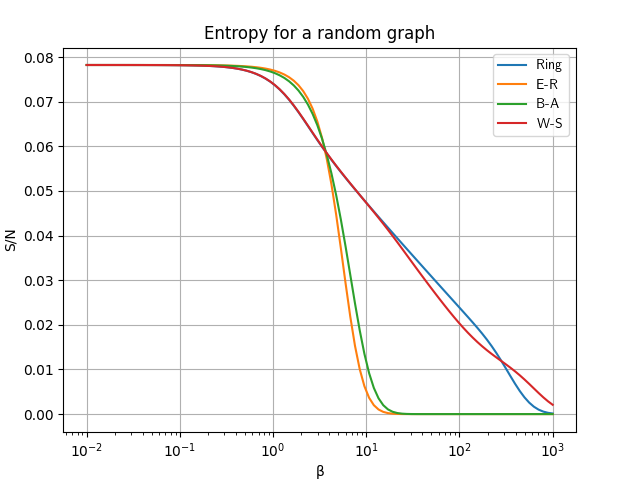
\includegraphics[width=0.75\linewidth]{image/random_graph.png}
    \caption{Plot of the network's entropy per node as a function of $\beta$ for different network types with $50$ nodes: a ring graph (blue), a Erd\H{o}s-Rényi (E-R) random graph with connectivity probability $0.7$ (orange), a Barab\'asi-Albert (B-A) scale-free graph with parameter $m=3$ (green), and a Watts-Strogatz (W-S) small world graph with parameter $K=3$ and rewire probability 0.2 (red). The x-axis has a logarithmic scale. For large $\beta$ the entropy tends to zero far all the networks.}
    \label{fig:ER-BA-WS}
\end{figure}

Using the density matrix, we can introduce also other thermodynamics quantities like the Helmoltz free energy $F = -\frac{1}{\beta} \ln Z$.


A possible interpretation of this density matrix is given by De Domenico \cite{De_Domenico_2020}.
Consider a network composed of $N$ nodes, encoded in the adjacency matrix $A$. Each node can be associated with a  value $n_i$ representing a property of the network, like the number of particles in the node in a diffusion model. 
The evolution of these variables is governed by the control operator $\hat L$. 

The network can be described using the Dirac notation. Let be $\ket{\psi} = \sum_i n_i \ket{i}$ the state of the system, where $\ket{i}$ is the canonical vector identifying the node $i$. The set $\{\ket{i}\}_{i=0}^N$ forms an orthogonal basis, satisfying $\braket{i}{j} = \delta_{ij}$, where $\delta_{ij}$ is the Kronecker delta.

The dynamics can be written as
\begin{equation} \label{time_evolution}
    \partial_t \ket{\psi(t)} = - \hat L \ket{\psi(t)},
\end{equation}
with the solution
\begin{equation}
    \ket{\psi(t)} = \hat G(t,0) \ket{\psi(0)}
\end{equation}
where $\hat G(t,0) = e^{-t\hat L}$ is the propagator and $\ket{\psi(0)}$ is the initial state. 

Since $\hat L$ is Hermitian, the propagator can be diagonalized in the orthogonal basis $\{\ket{v_\lambda}\}_\lambda$ of eigenvectors of the control operator
\begin{equation}\label{diagonal_propagator}
    \hat G(t,0) = \sum_\lambda e^{-t\lambda} \ket{v_\lambda}\bra{v_\lambda} = \sum_\lambda e^{-t\lambda} \hat \sigma_\lambda,
\end{equation}
where $\hat \sigma_\lambda$ is the projection over the left and right eigenvectors with the $\lambda$ eigenvalue. The operators do not depend on time, they are constant along the process, only the eigenvalues change.

The system relaxes to a stationary state $\ket{\psi_0}$ corresponding to the zero eigenvector.
We consider the system in the initial state $\ket{\psi} = \ket{\psi_0} + \ket{\Delta\psi}$, where $\ket{\Delta\psi}$ is a small perturbation relative to the stationary state. The initial perturbation can be decomposed as $\ket{\Delta\psi_0} = \sum_i \Delta_i \ket{i}$.
The time evolution of the state becomes
\begin{equation}
    \ket{\psi(t)} = G(t,0) \ket{\psi(0)} = \ket{\psi_0} + G(t,0)\ket{\Delta\psi} = \ket{\psi_0} + \ket{\Delta\psi(t)}
\end{equation}
with $\ket{\Delta\psi(t)} = e^{-t\hat L} \ket{\Delta \psi}$.

Since the stationary component is constant in time, we focus on the perturbation. 
The value of the perturbation at node $j$ at time $t$ is
\begin{equation}
    \braket{j}{\Delta\psi(t)} = \bra{j} e^{-t\hat L} \ket{\Delta\psi} =\sum_\lambda \bra{j} e^{-t\lambda} \hat \sigma_\lambda\ket{\Delta\psi} = \sum_i  \sum_\lambda \Delta_i e^{-t\lambda} \bra{j}  \hat \sigma_\lambda \ket{i}.
\end{equation}
We have used equation \eqref{diagonal_propagator} and the definition of the perturbation.
This equation shows that the perturbation travels through $N$ different streams, one for each $\sigma_\lambda$, with the stream's size $\Delta_i e^{-t\lambda}$. If $\Delta_i e^{-t\lambda} > 0$ the stream is active; if $\Delta_i e^{-t\lambda} = 0$ it is inactive. Negative stream coefficients imply an inverted flux from $j$ to $i$.
Sometimes, the dynamics traps part of the perturbation in a specific node. The trapped perturbation's size can be compute as
\begin{equation}
    T = \sum_i  \sum_\lambda \Delta_i e^{-t\lambda} \bra{i}  \hat \sigma_\lambda \ket{i} 
\end{equation} 

Assuming maximal uncertainty in the perturbation, obtainable when $\Delta_i = \Delta$, the equation reduces to
\begin{equation}
    T = \Delta \sum_i e^{-t\lambda} \bra{i}  \hat \sigma_\lambda \ket{i} = \Delta \Tr [\hat G(t,0)]
\end{equation}

Since the trapped perturbation regulates the stream's sizes, it can be responsible for the generation of the streams itself. 
Thus, we can define a density matrix 
\begin{equation}
    \hat \rho_t = \frac{1}{T} \Delta e^{-t\hat L} =  \frac{1}{Z} e^{-t\hat L},
\end{equation}
where $Z = \Tr[e^{-t\hat L}] $ is the partition function.
This density matrix can be interpreted as the probability that the perturbation will flow through a specific stream $\hat \sigma_l$ in the ensemble of all the possible streams \cite{De_Domenico_2020}.

The complexity of information streams can be quantified by the Von Neumann entropy.
When the information dynamics is described by a single information stream, a pure state, entropy is zero.
In contrast, as the information dynamics becomes more complex and diverse, the number of information streams increases, resulting in higher entropy.

\subsection{Kullback-Liebler and Jensen-Shannon Divergences}
Starting from the concept of entropy, we can also introduce the Kullback-Liebler (KL) divergence or relative entropy \cite{K-L_divergence} as
\begin{equation}\label{KL_divergence}
    D_{KL}(\hat \rho || \hat \sigma) = \Tr \left[\hat \rho \ln\left(\frac{\hat\sigma}{\hat\rho}\right)\right].
\end{equation}
It measure the close is the distribution $\hat \sigma$ to reproduce a event with real distribution $\hat \rho$. 
The KL divergence is always non negative and it equals zero when $\hat \rho = \hat \sigma$. It is not symmetric an unbounded \cite{J-S_divergence}.

It can be used to make comparisons between networks. Moreover, this concept we can be applied to the reconstruction of network starting from real data using the maximum likelihood estimation: it is to find the best model that reproduce the experimental data. In fact, the maximum likelihood estimation can be apply minimizing the Kullback-Liebler divergence between chosen network models and the dataset \cite{De_Domenico_2016}. This opens the door to the application of machine learning technique in complex network.


However the Kullback-Liebler divergence is not symmetric, therefore it can not be use as a metric. 
But we can symmetrize introducing the Jensen-Shannon (JS) divergence \cite{J-S_divergence} as
\begin{equation}\label{JS_metric}
    \mathcal{D}_{JS}(\hat\rho||\hat\sigma) =  \frac{1}{2}D(\hat \rho || \hat \mu) + \frac{1}{2}D(\hat \sigma || \hat \mu) = S(\hat\mu)-\frac{1}{2}\left[S(\hat\rho) + S(\hat\sigma)\right],
\end{equation}
where $\hat\mu =\frac{1}{2}(\hat\rho+\hat\sigma)$. 
\begin{figure}[ht!]
    \centering
    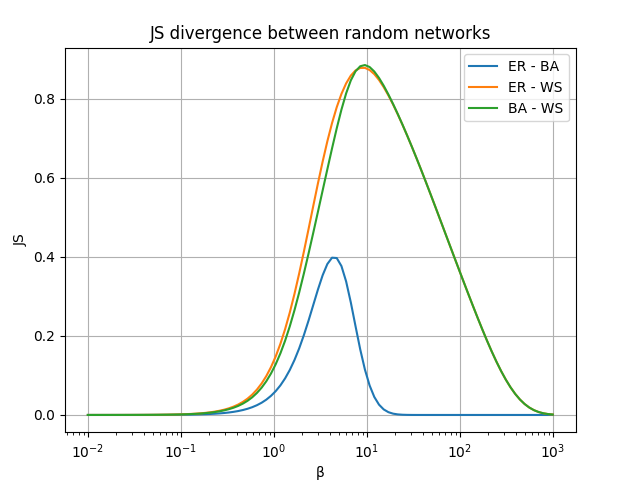
\includegraphics[width=0.75\textwidth]{image/JS_divergence.png}
    \caption{Plot of the KL divergence as a function of $\beta$ between different network types with $50$ nodes: a Erd\H{o}s-Rényi (E-R) random graph with connectivity probability $0.7$ and a Barab\'asi-Albert (B-A) scale-free graph with parameter $m=3$ (blue); a Erd\H{o}s-Rényi (E-R) random graph with connectivity probability $0.7$ and Watts-Strogatz (W-S) small world graph with parameter $K=3$ and rewire probability 0.2 (orange); a Barab\'asi-Albert (B-A) scale-free graph with parameter $m=3$ and a Watts-Strogatz (W-S) small world graph with parameter $K=3$ and rewire probability 0.2 (green). The x-axis has a logarithmic scale.The ER and BA networks are closer respect to a WS network. The divergence is maximum around $\beta = 10$.}
    \label{Fig:JS_divergence}
\end{figure}

The JS divergence is a bounded function \cite{J-S_divergence}
\begin{equation}
    0 \geq \mathcal{D}_{JS}(\hat\rho||\hat\sigma) \geq 1.
\end{equation}
$\left(\mathcal{D}_{JS}\right)^{\frac{1}{2}}$ defines a metric: it is symmetric, positive define, and hold the triangular inequality \cite{Jensen-Shannon_divergence}. 

%It has been use successfully to measure the distance between the layer of a multilayer network in order to aggregate them and eliminate the redundant layers \cite{multilayer}.
It has been use successfully to measure the distance between the network in order to aggregate them \cite{multilayer}.

Figure \ref{Fig:JS_divergence} shows the Jensen-Shannon divergence between an Erd\H{o}s-Rényi (E-R) random graph, a Barab\'asi-Albert (B-A) scale-free graph and a Watts-Strogatz (W-S) small-sworld graph \footnote{The python scripts can be found in the GitHub page of the author at the link: \url{https://github.com/ShqemzaMatteo/Master_thesis}}.

\chapter{Lindblad Master Equation}\label{C_Lindblad}
Before exploring the following chapter, it is useful to introduce the Lindblad master equation, also called Gorini-Kossakowski-Sudarshan-Lindblad equation \cite{Lindblad,G_K_S}. This equation was introduced to explain the behavior of an open quantum system, namely a quantum system in contact with the environment. This is important because the Schrödinger equation applies only to closed systems which are idealized and not realistic: all the quantum experiment we can build are susceptible to the external environment.
In this way we can recover and justify the basic assumption physicists do in quantum statistical mechanics.

The model investigates the evolution of a quantum system coupled to a Markovian environment, the interaction has no memory of the past.  
The Schrödinger equation requires an unitary time operator that does not allow energy dissipations. In contrast, the time operator of Lindblad master equation permits the system to dissipate energy with the surrounding. 
Despite this, the Lindblad dynamics remains trace preserving and completely positive.

\section{Derivation of the formula}
We show the derivation of the Lindblad equation following \cite{Manzano,Breuer-Petruccione}.
First, let $\mathcal{H}_T$ be the Hilbert space of the system and the environment combined, that can be divided between the Hilbert spaces $\mathcal{H}$ of the proper system and $\mathcal{H}_E$ of the environment. The combined system is a quantum closed system and evolves following the Von Neumann equation $\partial_t\hat\rho_T(t) = -i[\hat H_T,\hat\rho_T(t)]$, where $\hat H_T$ is the Hamiltonian of the total universe.
Since we are interesting only in the system's dynamics without the environment, we can trace out the degrees of freedom associated with it, obtaining $\hat\rho(t) = \Tr_E[\hat\rho_T]$. The total Hamiltonian can be separated as $H_T = H \otimes \mathbb{I}_E + \mathbb{I}_S \otimes H_E + \alpha H_I$, where $H$ is the Hamiltonian of the system, $H_E$ the Hamiltonian of the environment and $H_I$ is the interaction Hamiltonian, $\alpha$  measure the strength of the interaction.
It is useful to work in the interaction pictures where the operators becomes
\begin{equation}
    \tilde O(T) = e^{i(\hat H+\hat H_E)t}\hat O e^{-i(\hat H+\hat H_E)t},
\end{equation}
and the Von Neumann equation reduces to 
\begin{equation}\label{C_interacting_picture}
    \frac{d\tilde\rho_T(t)}{dt}= -i\alpha\left[\tilde H_I(t),\tilde\rho_T(t)\right].
\end{equation}  

The solution to \eqref{C_interacting_picture} is 
\begin{equation}\label{interacting_picture_exact_solution}
    \tilde\rho_T(t) = \tilde\rho_T(0) -i\alpha\int_{0}^{t}ds\left[\tilde H_I(s),\tilde\rho_T(s)\right].
\end{equation}

Even though the equation \eqref{interacting_picture_exact_solution} has an exact solution, it is complicate to compute. To simplify the calculation, we can introduce the \eqref{interacting_picture_exact_solution} into the \eqref{C_interacting_picture} giving
\begin{eqnarray}
    \frac{d\tilde\rho_T(T)}{dt}= -i\alpha\left[\tilde H_I(T),\tilde\rho_T(0)\right] -\alpha^2 \int_{0}^{t}ds\left[\tilde H_I(t),\left[\tilde H_I(s),\tilde\rho_T(s)\right]\right]
\end{eqnarray}

Apply this method again, we obtain
\begin{equation}
    \frac{d\tilde\rho_T(T)}{dt}= -i\alpha\left[\tilde H_I(T),\tilde\rho_T(0)\right] -\alpha^2 \int_{0}^{t}ds\left[\tilde H_I(t),\left[\tilde H_I(s),\tilde\rho_T(t)\right]\right] + O(\alpha^3)
\end{equation}
Now, we make an approximation: we consider the strength of the interaction $\alpha$ weak, in this way we can neglect the last term.
Now we can trace out the environment obtaining
\begin{equation}\label{trace_C_interacting_picture}
    \frac{d\tilde\rho}{dt} = -i\alpha\Tr_E\left[\tilde H_I(T),\tilde\rho_T(0)\right] -\alpha^2 \int_{0}^{t}ds \Tr_E\left[\tilde H_I(t),\left[\tilde H_I(s),\tilde\rho_T(t)\right]\right].
\end{equation}

However, the equation \eqref{trace_C_interacting_picture} still depends on the total density matrix. To proceed, we make two more assumptions. First, we consider the initial state of the universe as a separable state $\hat\rho_T(0)=\hat\rho(0)\otimes \hat\rho_E(0)$. This holds if the system is just been put in contact with the environment or if the correlation between the system and the environment is short-lived. This is called Born approximation. 
Second, we consider the environment to be in a thermal state 
\begin{equation}
    \hat\rho_E(0) = \frac{e^{-\hat H_E/T}}{\Tr\left[e^{-\hat H_E/T}\right]},
\end{equation}
where $T$ is the temperature (the Boltzmann constant $k_B = 1$).
Moreover, without loss of generality, we can write the interaction Hamiltonian in the form
\begin{equation}
    \hat H_I(t) = \sum_i \hat S_i\otimes \hat E_i,
\end{equation}
where $\hat S_i$ is an operator acting on $\mathcal{H}$ (is not a spin operator) and $\hat E_i$ is an operator acting on $\mathcal{H_E}$. After this assumption, the equation \eqref{trace_C_interacting_picture} becomes
\begin{equation}
    \begin{split}
        \frac{d\tilde\rho}{dt} =&-i\alpha\sum_i\left(\tilde S_i(t)\tilde \rho(0)\Tr_E\left[\tilde E_i(t)\tilde\rho_E(0)\right] - \tilde \rho(0)\tilde S_i(t)\Tr_E\left[\tilde\rho_E(0)\tilde E_i(t)\right]\right) \\ 
        &-\alpha^2 \int_{0}^{t}ds \Tr_E\left[\tilde H_I(t),\left[\tilde H_I(s),\tilde\rho(t)\otimes\tilde\rho_E(t)\right]\right].
    \end{split}
\end{equation}

The first term on the r.h.s. vanishes because $ \Tr_E\left[\tilde E_i(t)\tilde\rho_E(0)\right] = \left<E_i(t)\right>$ can be considered as zero. 
It may seem strange, however, if it does not vanish, we can always redefine the environmental Hamiltonian as $\hat E'_i = \hat E_i - \left<E_i(t)\right>$. The extra term is a constant and does not modify the Von Neumann equation.
The second term requires more stronger assumption: since $\alpha$ is small, the system and the environment should remain uncorrelated throughout the evolution, that is the timescale of the correlation should be much shorter than the timescale of the system. Thus, we can consider that the total density matrix is always separable, with the environment in the thermal state.
Nevertheless, the equation is still not markovian. To add this property, we can extend the upper limit of the integration to infinity with no real change in the outcome. Then, changing the integral variable to $t - s$, we arrive to 
\begin{eqnarray}\label{C_markovian}
    \frac{d\tilde \rho(t)}{dt} = -\alpha^2 \int_0^\infty ds \Tr_E\left[\tilde H_I(t),\left[\tilde H_I(t-s),\tilde\rho(t)\otimes\tilde\rho_E(t)\right]\right].
\end{eqnarray}
This is called Redfield equation \cite{Redfield}.
This is the Markov approximation, which is justified if the timescale over which the state of the system varies appreciably is large compared to the timescale over which the reservoir correlation functions decay. The sum of approximations made before are called Born-Markov approximation \cite{Breuer-Petruccione}.

The equation \eqref{C_markovian} can generate a negative density matrix. To exclude this possibility, we consider a superoperator $\mathbb{H} A = \left[H,A\right]$, with $A$ a general operator. The eigenvectors of the superoperator generate a complete basis of the space $\{\hat S_i(\omega)\}$ of the bounded operators acting on the Hilbert $\mathcal{H}$, they satisfy the condition
\begin{equation}
    \mathbb{H}\hat S_i(\omega) = -\omega \hat S_i(\omega) \qquad \mathbb{H}\hat S_i^\dagger(\omega) = \omega \hat S_i^\dagger(\omega).
\end{equation}
Here, $\omega$ indicates the energy difference after the operator $\hat A_i(\omega)$ has acted.
It satisfies the relations
\begin{equation}
    \begin{split}
        e^{i\hat H_St}\hat A(\omega)e^{-i\hat H_St} = e^{-i\omega t}\\
        e^{i\hat H_St}\hat A^\dagger(\omega)e^{-i\hat H_St} = e^{i\omega t}\\
    \end{split}
\end{equation}
We can decompose the operators $S_i$ as $\hat S_i = \sum_\omega \hat S_i(\omega)$.
To apply this decomposition in \eqref{C_markovian}, we need to go back to the Schrödinger picture for the Hamiltonian acting on the proper system. Using $\tilde S_i(\omega)=e^{i\hat Ht}\hat S_i(\omega)e^{-i\hat H t}$, we obtain the Hamiltonian in the interacting picture
\begin{equation}\label{eigen_Hamiltonian}
    \tilde H_i(t) = \sum_{i\omega} e^{-i\hat Ht}\hat S_i(\omega) \otimes \tilde E_i (t)= \sum_{i\omega} e^{i\hat Ht}\hat S_i^\dagger(\omega) \otimes \tilde E_i (t)
\end{equation}

After expanding the commutators in \eqref{C_markovian}, we substitute the decomposition for $\hat S_k(\omega)$. Using the cyclic property of the trace and the fact that $\Tr[\hat H_e,\hat\rho_E(0)]=0$, we arrive at the result
\begin{equation}\label{c_substitue}
    \frac{d\tilde\rho(t)}{dt} = \sum_{\omega,\omega',i,j}e^{i(\omega-\omega')t}\Gamma_{ij}\left[\hat S_j(\omega)\tilde\rho(t),\hat S_i^\dagger(\omega')\right]+ e^{-i(\omega-\omega')t}\Gamma_{ji}^\dagger\left[\hat S_j(\omega),\tilde\rho(t)\hat S_i^\dagger(\omega')\right],
\end{equation}
where $\Gamma_{kl}(\omega)$ contains the effect of the environment and it is defined as
\begin{equation}\label{environment_coefficients}
    \Gamma_{ij}(\omega) = \int_{0}^{\infty}ds e^{i\omega s}\Tr\left[\tilde E_i^\dagger(t)\tilde E_j(t-s)\hat\rho_E(0)\right]
\end{equation}
where the operator $\tilde E_j(t)=e^{i\hat H_E t}\hat E_j e^{-i\hat H_E t}$ is in the interaction picture. It does not depend on time since the environment is in a stationary state and the correlation function of the environment decay extremely fast.

Now, we make the final assumption: we consider the system in the rotating wave approximation. The terms proportional to $|\omega-\omega'| >> \alpha^2$ will oscillate much faster than the timescale of the system; thus, they do not contribute to the evolution of the system. In the low-coupling regime, $\alpha\rightarrow 0$, we can consider that only the resonant terms, $\omega=\omega'$, contribute to the dynamics and remove all the others. Therefore, the equation \eqref{c_substitue} reduces to
\begin{eqnarray}\label{C_rotating_wave}
    \frac{d\tilde\rho(t)}{dt} = \sum_{\omega,i,j}\Gamma_{ij}\left[\hat S_j(\omega)\tilde\rho(t),\hat S_i^\dagger(\omega)\right]+\Gamma_{ji}^\dagger\left[\hat S_j(\omega),\tilde\rho(t)\hat S_i^\dagger(\omega)\right].
\end{eqnarray}

The operators $\Gamma_{ij}(\omega)$ are not necessarily Hermitian. Thus, we divide them into the Hermitian and not Hermitian parts, $\Gamma_{ij}(\omega) =\frac{1}{2}\gamma_{ij}(\omega)+i\pi_{ij}(\omega)$, respectively
\begin{equation}
    \begin{split}
        \gamma_{ij}(\omega) &=   \Gamma_{ij}(\omega) + \Gamma_{ij}^\dagger(\omega) = \int_{-\infty}^\infty ds e^{i\omega s}\Tr\left[\left\{\tilde E_i^\dagger(t),\tilde E_j(t-s)\right\}\hat\rho_E(0)\right]\\
        \pi_{ij}(\omega) &= \frac{-i}{2}\left(\Gamma_{ij}(\omega)-\Gamma_{ij}^\dagger(\omega)\right)\int_{-\infty}^\infty ds e^{i\omega s}\Tr\left[\left[\tilde E_i^\dagger(t),\tilde E_j(t-s)\right]\hat\rho_E(0)\right]\\
    \end{split}
\end{equation}

Inserting them into the equation \eqref{C_rotating_wave} and returning to the Schrödinger picture, we obtain
\begin{equation}\label{general_Lindblad_equation}
    \frac{d}{dt}\hat\rho = -i\left[\hat H + \hat H_{LS},\hat\rho\right] + \sum_{i,j,\omega} \gamma_{ij}(\omega) \left(\hat S_i(\omega) \hat\rho \hat S^\dagger_j(\omega) - \frac{1}{2}\left\{ \hat S^\dagger_i(\omega)\hat S_j(\omega), \hat\rho\right\} \right),
\end{equation}
where $\hat H_{LS} = \sum_{\omega,i,j} \pi_{ij}(\omega)\hat S^\dagger_i(\omega)\hat S_j(\omega)$ is called Lamb shift Hamiltonian and it adjusts the energy levels due to thee interaction with the environment. The equation \eqref{general_Lindblad_equation} is the general version of the Markovian master equation. The matrix $\gamma(\omega)$ must be positive define, although the trace preserving of the dynamics is not guaranteed.

If the matrix $\gamma(\omega)$ can be diagonalized, namely exist a diagonal matrix $D=\hat O \gamma(\omega) \hat O^\dagger$ with $\hat O$ a unitary operator, and considering the simplest case of just one frequency $\omega$ then we can write the Lindblad-Gorini-Kossakowski-Sudarshan master equation as
\begin{equation}\label{Lindbladian}
    \frac{d}{dt}\hat\rho =\mathcal{L}\left[\hat\rho\right] = -i\left[\hat H+\hat H_{LS},\hat\rho\right] + \sum_k \gamma_k \left(\hat J_k \hat\rho \hat J^\dagger_k - \frac{1}{2}\left\{ \hat J^\dagger_k\hat J_k, \hat\rho\right\} \right).
\end{equation}
The operator $\hat J_k= \sum_i O_{ki} \hat S_{i}$ are called jump operators, the superoperator $\mathcal{L}$ is called Lindblad superoperator and $\gamma_i$ are the damping rates. In the limit $\gamma_k = 0$ the Von Neumann equation is recovered.



\section{Properties of the Lindblad equation}
The Lindblad master equation satisfies some important properties.
The Lindblad master equation defines a set of dynamical maps $\phi_t\left(\hat\rho\right)= e^{\mathcal{L}t}\hat\rho(0)$ on the space of density matrices such that
\begin{equation}
    \hat\rho(t) = \phi_t\left(\hat\rho(0)\right).
\end{equation}
These maps have the semigroup property, that is,
\begin{equation}
    \phi_s\left(\phi_t\left(\hat\rho(0)\right)\right)=\phi_{t+s}\left(\hat\rho(0)\right)
\end{equation}

The Lindblad master equation is the most general form for the generator of a quantum dynamical system. As a matter of fact, the Lindblad equation can also be derived starting from this assumption \cite{Breuer-Petruccione}.

The Lindblad master equation is invariant under the following transformations \cite{Breuer-Petruccione}:
\begin{itemize}
    \item Unitary transformation of the Lindblad operator:
        \begin{equation}
            \sqrt{\gamma_i}\hat J_i \rightarrow \sqrt{\gamma_i'}\hat J_i' = \sum_j u_{ij}\sqrt{\gamma_j}\hat J_j
        \end{equation}
        where $u_{ij}$ is an unitary matrix.
    \item Inhomogeneous transformation:
        \begin{equation}
            \begin{split}
                \hat J_i &\rightarrow \hat J'_i = \hat J_i + a_i\\
                \hat H_I &\rightarrow \hat H' = \hat H + \frac{1}{2i}\sum_j\gamma_j\left(a^*_j\hat J_j -a_j\hat J_j^\dagger\right)
            \end{split}
        \end{equation}
        where $a_i \in\mathbf{C}$ and $b \in \mathbf{R}$.
\end{itemize}
The last transformation allows us to always choose a traceless jump operator.

Lastly, we can prove that the dynamics \eqref{Lindblad_master_equation} conserve $\Tr[\hat\rho]$. As a matter of fact, the derivative along time of it is
\begin{equation}\label{Lindblad_master_equation}
    \frac{d}{dt}\Tr[\hat\rho] = \Tr\left[-i\left(\hat H\hat\rho - \hat\rho\hat H \right) +  \hat J_k \hat\rho \hat J_k^\dagger -\frac{1}{2} \left(\hat L\hat\rho + \hat\rho\hat L\right)\right] = 0,
\end{equation}
proved using the cyclic property of the trace. 
However, it does not conserve the purity $\Tr\left[\hat\rho^2\right]$ that decreases \cite{Manzano}. 


\section{Stationary distribution}
The Lindblad equation allows for a stationary distribution that satisfies the condition
\begin{equation}
    \mathcal{L}\hat\rho = 0.
\end{equation}

In the previous section, we assumed that the environment is in a Gibbs state. Now, consider that the damping parameter satisfies the relation
\begin{equation}\label{C_gamma}
    \gamma_{ij}(-\omega) = e^{-\beta \omega}\gamma_{ij}(\omega)
\end{equation}
which is called KMS condition \cite{Breuer-Petruccione}.
If this condition is satisfied, it can be proven that the stationary distribution is equal to the Gibbs states \cite{Breuer-Petruccione}
\begin{equation}
    \hat\rho^* = \frac{e^{-\beta \hat H}}{\Tr\left[e^{-\beta \hat H}\right]}.
\end{equation}

If the spectrum of the Hamiltonian $H = \sum_n \epsilon_n\ket{n}\bra{n}$ is not degenerate, it gives rise to a closed equation for the population 
\begin{equation}
    P(n,t) = \bra{n}\hat\rho(t)\ket{n}
\end{equation}
Thus, the dynamics decouple the diagonal and off-diagonal terms. The former are governed by the Pauli master equation
\begin{equation}\label{to_Fermi_golden_rule}
    \frac{dP(n,t)}{dt} = \sum_m \left[ W(n|m)P(m,t) - W(m|n)P(n,t)\right]
\end{equation}
with time independent transition rate
\begin{equation}
    W(n|m) = \sum_{ij} \gamma_{ij}(\epsilon_n -\epsilon_m)\bra{n}\hat J_i(t)\ket{m} \bra{m}\hat J_j(t)\ket{n}. 
\end{equation}

Using the equation \eqref{C_gamma} and considering the l.h.s. of the equation \eqref{to_Fermi_golden_rule} , we obtain the Fermi Golden rule
\begin{equation}
    W(n|m)e^{-\beta \epsilon_n} = W(m|n) e^{-\beta \epsilon_m}
\end{equation}
which is nothing other that a detailed balance condition with stationary distribution
\begin{equation}
    \hat\rho = \frac{1}{Z}e^{-\beta \hat H}
\end{equation}
with $\beta$ the inverse temperature of the environment and $Z = \Tr\left[e^{-\beta \hat H}\right]$ is the partition function.

\section{Entropy production}

\section{Caldeira-Leggett model}

The Caldeira-Leggett model was proposed in 1983 to reproduce the Brownian motion via a quantum process.
It study the dynamics of a particle in contact with a thermal bath made by a set of harmonic oscillator.
However, the model present the Markovian propery only in the high temperature weak coupling limit and a not Markovian one in otherwise.

The free Hamiltonian of the particle is
\begin{equation}
    H_S = \frac{\hat p^2}{2m} + V(\hat q),
\end{equation}
where $\hat p$ is the momentum operator and $V(\hat q)$ is the potential.

The particle is in contact with the bath composed by N harmonic oscillator. The Hamiltonian is
\begin{equation}
    H_E = \sum\Omega_n(\hat b_n^\dagger\hat b_n+\frac{1}{2})= \sum_n \left(\frac{p_n^2}{2m_n}+ \frac{1}{2}m_n\Omega_n^2q_n^2\right).
\end{equation}
where $\hat b_n^\dagger$ and $\hat b_n$ are respectively the creation and annihilation operators of the bath, and $p_n$ and $q_n$ the momentum and position operator of the oscillators of bath.

The interaction Hamiltonian is given by
\begin{equation}
    H_I = \hat q\sum_n k_n \hat q_n = - \hat B \hat q = \hat q \sum_n k_n\frac{1}{\sqrt{2m_n\Omega_n}}\left(\hat b+ \hat b^\dagger\right)
\end{equation}
where $\hat B$ is the bath operator.

We need to add a counterterm 
\begin{equation}
    H_C = \sum_n \frac{\hat q^2}{2m_n\Omega_n^2}. 
\end{equation}

Starting from equation \eqref{C_markovian} in the Schrödinger pictures
\begin{equation}
    \frac{d \rho(t)}{dt} = i\left[\hat H_S+ \hat H_C, \hat\rho(t)\right] -\int_0^\infty ds \Tr_E\left[\hat H_I(t),\left[\hat H_I(t-s),\hat\rho(t)\otimes\hat\rho_E(t)\right]\right],
\end{equation}

We can rewrite it using the correlation relations of the bath
\begin{equation}
    D(s) =i \left<\left[\hat B, \hat B^\dagger(t-s)\right]\right> \qquad D'(s) = \left<\left\{\hat B, \hat B^\dagger(t-s)\right\}\right>
\end{equation}
into the formula 
\begin{equation}\label{CL_master_eq}
    \frac{d \rho(t)}{dt} = -i\left[\hat H_S+ \hat H_C, \hat\rho(t)\right] -\int_0^\infty ds \frac{i}{2} D(s)\left[\hat q, \left\{\hat q(-s), \hat \rho(t)\right\}\right] - \frac{1}{2} D'(s)\left[\hat q, \left[\hat q(-s), \hat\rho(t)\right]\right]  
\end{equation}

Using the spectral density
\begin{equation}
    J(\Omega) = \sum_n \frac{k_n^2}{2m_n\Omega}\delta(\Omega-\Omega_n)
\end{equation}
we can rewrite the correlation as
\begin{equation}
    D(s) = 2\int_0^\infty d\Omega J(\Omega) \sin\Omega s \qquad D'(s) = 2\int_0^\infty d\Omega J(\Omega) \coth\left(\frac{\Omega}{2k_BT}\right)\cos\Omega s.
\end{equation}

We can simplify further the equation \eqref{CL_master_eq} looking at the $\hat q(-s)$, indeed, it can be written as 
\begin{equation}
    \hat q(-s) = e^{-i\hat H_S s} \hat q e^{i\hat H_S s} \approx \hat q- i\left[\hat H_S, \hat q\right]s = \hat q - \frac{\hat p}{m}s 
\end{equation}

Inserting it into \eqref{CL_master_eq} we obtain
\begin{equation}
    \begin{split}
        \frac{d \rho(t)}{dt} = & -i\left[\hat H_S+ \hat H_C, \hat\rho(t)\right] -\frac{i}{2}\int\limits_0^\infty ds  D(s)\left[\hat q, \left\{\hat q, \hat \rho(t)\right\}\right]\\
        &+ \frac{i}{2m}\int_0^\infty ds \, sD(s)\left[\hat q, \left\{\hat p, \hat \rho(t)\right\}\right] - \frac{1}{2}\int_0^\infty ds D'(s)\left[\hat q, \left[\hat q, \hat\rho(t)\right]\right]\\
        & +\frac{1}{2m}\int_0^\infty ds \; sD'(s)\left[\hat q, \left[\hat p, \hat\rho(t)\right]\right].\\
    \end{split}  
\end{equation}

Then, we solve the integral in the high temperature limit: the first term give us the exactly the counter term  $-i\left[\hat H_C, \hat \rho\right]$, the second becomes $-\frac{i\gamma}{2}\left[\hat q, \left\{\hat p,\hat \rho(t)\right\}\right]$, the third becomes $2m \gamma k_BT\left[\hat q,\left[\hat q,\hat\rho(t)\right]\right]$ and the last give us $\frac{2\gamma k_BT}{\Omega}\left[\hat q, \left[\hat p, \hat \rho\right]\right]$ which is negligible in the limit $\Omega \rightarrow \infty$ that we are dealing with.

We have reached the Caldeira-Leggett master equation
\begin{equation} \label{Caldeira-Leggett_master_equation}
    \frac{d\hat\rho}{dt} = -i\left[\hat H_S, \hat\rho(t)\right]-\frac{i\gamma}{2}\left[\hat q, \left\{\hat p,\hat \rho(t)\right\}\right] - 2m \gamma k_BT\left[\hat q,\left[\hat q,\hat\rho(t)\right]\right]. 
\end{equation}
The Caldeira-Leggett master equation reminds of the Langevin equation where the second term is the dissipative one and the third describes the fluctuations.


\chapter{Quantum Network Master Equation}\label{C_Quantum_Network_Master_Equation}

In Chapter \ref{C_Density_Matrix} we introduced the concept of the density matrix for a network, derived from the communicability matrix. This quantity captures the correlations between the nodes in a random walk dynamics.

In this chapter, we aim to unify the two concept taken from the quantum realm we have introduced: the quantum walk and the network's density matrix.
Specifically, we analyze a quantum walk process subjected to thermal noise, from which we derive a stationary distribution which coincides with the network's density matrix. 
The interaction between the quantum system and the thermal noise are treated as Markovian, meaning they do not depend on the past, thus, we study them using the Lindblad master equation.

\section{Quantum Stochastic Random Walk}\label{C_Quantum Stochastic Walk}

One of the early approaches to a Open Quantum Walk on network was proposed by Whitfield, Rodr\'iguez-Rosario and Aspuru-Guzik. \cite{QSW}. They defined a quantum walk on network in contact with a thermal bath with the dynamics described by a Lindblad master equation. In this framework, the jump operators are proportional to the adjacency  matrix $A_{ij}$ of the network. The thermal bath introduces noise into the dynamics, causing it which to deviate from the  Von Neumann equation \eqref{Von Neumann equation}. The system dissipation is reminiscent of the classic random walk.

Let us consider a quantum walk on a network $G(N,M)$, the system in contact with a thermal bath that randomly interact with modifying the dynamic of the quantum particle.
Let us introduce a Hilbert space $\mathcal{H}$ with an orthonormal basis $\{\ket{i}\}_{i<N}$, where each element $\ket{i}$ corresponds to the node $i$, satisfying $\braket{i}{j}=\delta_{ij}$. The system is described by a density matrix $\hat \rho$ whose evolution follows the Lindblad master equation \eqref{Lindblad_master_equation}.
The Laplacian operator $\hat L$, defined as in equation \eqref{Laplacian_operator}, serves as the Hamiltonian $\hat H$, while the jump operators $\{\hat J_k\}_{k<M}$ represent the thermal jumps between two node linked together. For convenience, we will denote the jump operator with two indeces referring to the starting node $j$ and the ending node $i$ of the jump: therefore, the jumps operator are $\hat J_{ij} = \ket{i}\bra{j}$. The damping rates are $\gamma_{ij} =A_{ij}/d_i$, like the transition rates in the classical random walk \eqref{transition_rates}.
The master equation can be expressed as follows:
\begin{equation}\label{stochastic_lindblad_master}
    \frac{d}{dt}\hat \rho = -\frac{i}{2}\left[\hat L,\hat\rho\right] + \sum_{ij}\gamma_{ij}\left[\hat J_{ij} \hat\rho\hat J_{ij}^\dagger -\frac{1}{2} \left\{ \hat J_{ij}^\dagger \hat J_{ij}, \hat\rho\right\}\right],
\end{equation}
where $[\cdot,\cdot]$ and $\{\cdot,\cdot\}$ denote respectively the commutator and the anticommutator.
The equation \eqref{stochastic_lindblad_master} is composed by two distinct terms. The first term, also called coherent dynamics,  is given by
$\mathcal{L}^{qm}\left[\hat\rho(t)\right] = -i\left[H,\hat\rho\right]$ is equal to the quantum walk dynamics. In contrast, the second term, denoted as $\mathcal{L}^{cl}\left[\hat\rho(t)\right] = \sum_i \gamma_i \left(\hat J_i \hat\rho \hat J^\dagger_i - \frac{1}{2}\left\{ \hat J^\dagger_i\hat J_i, \hat\rho\right\} \right)$, called decoherent dynamics, encodes the dissipation. 
When $\gamma_{ij} = 0$ we recover the Von Neumann equation for the quantum walk \eqref{Von Neumann equation}. 
$\mathcal{L}\left[\hat\rho(t)\right]$ act as a superoperator in the space of the density matrix.

In the Fock-Liouville space, the quantum system evolves according the equation
\begin{equation}
    \sket{\rho(t)}  = U(t,0) \sket{\rho(0)}
\end{equation} 
where the evolution operator is defined as \cite{Domino}
\begin{equation}
    \begin{split}
        \hat U(t,0) = \exp&\left\{-it\left(\hat H\otimes\mathbb{I}-\mathbb{I}\otimes\hat H\right)\right.\\
        &+\left. t\sum_{ij}\gamma_{ij}\left[ \hat J_{ij}\otimes\hat J^\dagger_{ij}-\frac{1}{2}\hat J_{ij}\hat J^\dagger_{ij}\otimes\mathbb{I}-\frac{1}{2}\mathbb{I}\otimes\hat J_{ij}\hat J^\dagger_{ij}\right]\right\}.
    \end{split}
\end{equation}

The master equation \eqref{stochastic_lindblad_master} contains both the quantum and classical aspects of a random walk over a network. As a matter of fact, the classical random walk behavior emerges when we consider the evolution of the diagonal elements of the density matrix under the dissipative part alone. Let $\rho = \ket{k}\bra{k}$ represent the density matrix of a system localized at node $k$. Its evolution is given by
\begin{equation}
    \begin{split}
        \mathcal{L}^{cl}\ket{k}\bra{k} &= \sum_{ij}\gamma_{ij}\left[\hat J_{ij} \ket{k}\bra{k}\hat J_{ij}^\dagger -\frac{1}{2} \left\{ \hat J_{ij}^\dagger \hat J_{ij}, \ket{k}\bra{k}\right\}\right]\\
        %&= \sum_{ij}\left[\sqrt{A_{ij}}\ket{i}\braket{j}{a}\braket{a}{j}\bra{i}\sqrt{A_{ij}} -\frac{1}{2}\ket{i}\sqrt{A_{ia}}\braket{j}{j}\sqrt{A_{ia}}\braket{i}{a}\bra{a}\right.\\ 
        %&\quad \left. - \frac{1}{2} \ket{a}\braket{a}{i}\sqrt{A_{ia}}\braket{j}{j}\sqrt{A_{ia}}\bra{i}\right]\\
        &= \sum_{i}\left[\gamma_{ik} \ket{i}\bra{i} -\gamma_{ik}\ket{k}\bra{k}\right]\\
        &=\sum_{i} \left(\gamma_{ki} - \gamma_{ki}\delta_{ki}\right) \ket{i}\bra{i} = -\sum_i L_{ki} \ket{i}\bra{i}.
    \end{split} 
\end{equation} 
where $d_i$ is the degree of the node $i$.
This expression recovers the dynamics of the classical random walk over the network.
Next, considering the off-diagonal terms, their evolution is described by
\begin{equation}
    \begin{split}
        \mathcal{L}^{cl}\ket{k}\bra{l} &= \sum_{ij}\gamma_{ij}\left[\hat J_{ij} \ket{k}\bra{l}\hat J_{ij}^\dagger -\frac{1}{2} \left\{ \hat J_{ij}^\dagger \hat J_{ij}, \ket{k}\bra{l}\right\}\right]\\
        %&= \sum_{ij}\left[\sqrt{A_{ij}}\ket{i}\braket{j}{k}\braket{l}{j}\bra{i}\sqrt{A_{ij}} -\frac{1}{2}\ket{i}\sqrt{A_{ik}}\braket{j}{j}\sqrt{A_{ik}}\braket{i}{k}\bra{l}\right.\\ 
        %&\quad\left. - \frac{1}{2} \ket{k}\braket{l}{i}\sqrt{A_{ik}}\braket{j}{j}\sqrt{A_{ik}}\bra{i}\right]\\
        &= \sum_{j}\left[-\frac{1}{2} \gamma_{jk}\ket{k}\bra{l} - \frac{1}{2} \gamma_{jl}\ket{k}\bra{l}\right]\\
        &= -\ket{k}\bra{l}.
    \end{split} 
\end{equation}

The operator $\mathcal{L}^{cl}$ does not mix the diagonal terms with the off-diagonal ones, allowing us to separate the superoperator into two blocks: one for the diagonal element and the another for the off-diagonal ones.
Thus, the superoperator $\mathcal{L}^{cl}$ has a diagonal form with spectrum given by $\sigma^{cl} = -(\lambda_1,...,\lambda_N,1,...,1))$, where $\lambda_i$ are the eigenvalue of the Laplacian matrix \cite{Bruderer_Plenio}.
If the network satisfies the detailed balance condition \eqref{detail_condition}, the Laplacian matrix has a zero eigenvalue. Therefore, the superoperator $\mathcal{L}^{cl}$ will also have a zero eigenvalue indicating the presence of a stationary distribution.

\begin{comment}
    \begin{equation}
    \begin{split}
    \mathcal{L}^{qm}\ket{k}\bra{l} =& -i\hat L\ket{k}\bra{l} + i \ket{k}\bra{l}\hat L\\
    &=\frac{i}{2}\sum_{ij} - L_{ij}\ket{i}\braket{j}{k}\bra{l} + \ket{k}\braket{l}{i}\bra{j}\\
    &=\frac{1}{2}\sum_i -L_{ik} \ket{i}\bra{l} + \sum_i L_{li}\ket{k}\bra{i}\\
\end{split}
\end{equation}

Instead the diagonal terms
\begin{equation}
\begin{split}
\mathcal{L}^{qm}\ket{l}\bra{l} =& -i\hat L\ket{l}\bra{l} + i \ket{l}\bra{l}\hat L\\
&=\frac{i}{2}\sum_{ij} - L_{ij}\ket{i}\braket{j}{l}\bra{l} + \ket{l}\braket{l}{i}\bra{j}\\
&=\frac{1}{2}\sum_i -L_{il} \ket{i}\bra{l} + \sum_i L_{li}\ket{l}\bra{i} = 0\\
\end{split}
\end{equation}
\end{comment}

\subsection{Stationary distribution}

Following the proof of the stationary distribution in Chapter \ref{C_Lindblad}, we can find the stationary density matrix $\hat\rho^*$ for the quantum stochastic walk.
We will consider only the dissipative dynamics, which decouples the diagonal and off-diagonal terms. The evolution of the diagonal elements is described by:
\begin{equation}
    \frac{d}{dt}\rho_{ii} = \sum_j\left[\gamma_{ij}\rho_{jj}(t) - \gamma_{ji}\rho_{ii}(t)\right],
\end{equation}

The stationary distribution must satisfy the detail balance, namely
\begin{equation}
    \gamma_{ij}\rho_{jj}(t) = \gamma_{ji}\rho_{ii}.
\end{equation}
Because the damping rates fort this system are symmetric, the diagonal entries must be equal. 
Instead, considering the vector $\sket{\rho}$, the block corresponding to the off-diagonal part of $\mathcal{L}$ is already eigenstate with eigenvalue $1$. Thus, the off-diagonal terms must be equal to zero.
The stationary density matrix can then be expressed as
\begin{equation}\label{QSW_stationary_distribution}
    \hat\rho^* = \frac{1}{N}\begin{pmatrix}
        1&&0\\
        &\ddots&\\
        0&&1\\
    \end{pmatrix}.
\end{equation}
As discussed in chapter \ref{C_entropy_production}, the stationary density matrix has maximal Von Neumann entropy 
\begin{equation}
    S\left(\hat\rho^*\right) = \ln N.
\end{equation}

The density matrix \eqref{QSW_stationary_distribution} commutes with the Laplacian matrix, confirming that it is indeed the stationary density matrix for the dynamics described by \eqref{stochastic_lindblad_master}.

\begin{comment}
    Instead, adding also the coherent part, we need to go in the basis $\{\ket{\lambda}\}$ eigenvector of $\hat L$. 
    The decoherent part becomes
    \begin{equation}
    \begin{split}
    \mathcal{L}^{cl}\ket{\lambda}\bra{\lambda} &= \sum_{ij}\gamma_{ij}\left[\hat J_{ij} \ket{\lambda}\bra{\lambda}\hat J_{ij}^\dagger -\frac{1}{2} \left\{ \hat J_{ij}^\dagger \hat J_{ij}, \ket{\lambda}\bra{\lambda}\right\}\right]\\
        &= \sum_{ij}\gamma_{ij}\left[\ket{i}\braket{j}{\lambda}\braket{\lambda}{j}\bra{i} -\frac{1}{2}\ket{j}\braket{i}{i}\braket{j}{\lambda}\bra{\lambda} - \frac{1}{2}\ket{\lambda}\braket{\lambda}{j}\braket{i}{i}\bra{j} \right]\\
        & = \sum_{ij}\gamma_{ij}\left[|\braket{j}{\lambda}|^2\ket{i}\bra{i} -\frac{1}{2}\ket{j}\braket{j}{\lambda}\bra{\lambda} - \frac{1}{2}\ket{\lambda}\braket{\lambda}{j}\bra{j} \right]\\
        &= \sum_{ij}\left[\pi_{ij}\rho_j\ket{i}\bra{i} -\frac{\pi_{ij}}{2}\braket{j}{\lambda}\ket{j}\bra{\lambda} - \frac{\pi_{ij}}{2}\braket{\lambda}{j}\ket{\lambda}\bra{j} \right]
    \end{split}
\end{equation}
\end{comment}


\section{Quantum Network Master Equation}\label{C_quantum_network_master_equation}

The previous description for the noise in the quantum walk lacks a parameter that, in thermodynamics, correspond to the temperature. 
Thus, we propose another framework: instead of considering the jump operator as a transition between the nodes, we consider the thermal bath interaction in the energy states.
Let us retake the standard Lindblad equation \eqref{Lindbladian} with Hamiltonian $\hat H = \hat L$.
We introduce the basis $\{\ket{\lambda}\}_{\lambda}$ such that $\hat H = \sum_\lambda \lambda\ket{\lambda}\bra{\lambda} = \hat L$ is diagonal (the network must satisfy the detailed balance condition \eqref{detail_condition}).
We define the jump operator $\hat J_{\lambda\mu} = \ket{\lambda}\bra{\mu}$ as the jumps from the energy state $\ket{\mu}$ to the energy state $\ket{\lambda}$ obtaining the master equation
\begin{equation}\label{Lindblad_energy_jump}
    \frac{d}{dt}\hat\rho = -i\left[\hat L,\hat\rho\right] + \sum_{\lambda\mu} \gamma_{\lambda\mu} \left(\hat J_{\lambda\mu} \hat\rho \hat J^\dagger_{\lambda\mu} - \frac{1}{2}\left\{ \hat J^\dagger_{\lambda\mu}\hat J_{\lambda\mu}, \hat\rho\right\} \right),
\end{equation}
where the coefficients $\gamma_{\lambda\mu}$ indicate the probability of taking their respective jumps.

We assume that the dynamics will tend to a stationary distribution in the form of
\begin{equation}\label{pretended_stationary_distribution}
    \hat \rho^* = \frac{e^{-\beta\hat L}}{Z},
\end{equation}
with $Z = \Tr\left[e^{-\beta\hat L}\right]$ being the partition function.
The master equation for the stationary distribution \eqref{pretended_stationary_distribution} reduces to
\begin{equation}\label{cancel_master_equation}
    0 = -i\left[\hat H, \frac{e^{-\beta\hat L}}{Z}\right] + \sum_{\lambda\mu} \gamma_{\lambda\mu} \left(\hat J_{\lambda\mu}  \frac{e^{-\beta\hat L}}{Z} \hat J^\dagger_{\lambda\mu} - \frac{1}{2}\left\{ \hat J^\dagger_{\lambda\mu}\hat J_{\lambda\mu},  \frac{e^{-\beta\hat H}}{Z}\right\} \right).
\end{equation}
The first term on the r.h.s. vanishes since the commutator is zero.

Now, we analyze the dissipation terms independently.
The first one can be written as 
\begin{equation}\label{BCS_first_term}
        \sum_{\lambda\mu} \gamma_{\lambda\mu} \ket{\lambda}\bra{\mu}\frac{e^{-\beta\hat L}}{Z} \ket{\mu}\bra{\lambda} = 
        \sum_{\lambda\mu} \gamma_{\lambda\mu} \frac{e^{-\beta \epsilon_\mu}}{Z} \ket{\lambda}\bra{\lambda}.
\end{equation}
While the second becomes
\begin{equation}\label{BCS_second_term}
    \sum_{\lambda\mu} \gamma_{\lambda\mu}\left[\frac{1}{2}\ket{\mu}\braket{\lambda}{\lambda}\bra{\mu}\frac{e^{-\beta\hat L}}{Z} +\frac{1}{2}\frac{e^{-\beta\hat L}}{Z}\ket{\mu}\braket{\lambda}{\lambda}\bra{\mu}\right]= \sum_{\lambda\mu} \gamma_{\lambda\mu}\left[\frac{e^{-\beta \epsilon_\mu}}{Z}\ket{\mu}\bra{\mu}\right].
\end{equation}
Therefore, inserting the equations \eqref{BCS_first_term} and \eqref{BCS_second_term} into the master equation \eqref{cancel_master_equation}, we obtain the condition
\begin{equation}\label{Kirchhoff_law_energy}
    \sum_{\lambda\mu}\left[\gamma_{\lambda\mu}\frac{e^{-\beta \mu}}{Z} - \gamma_{\mu\lambda}\frac{e^{-\beta \lambda}}{Z}\right]\ket{\lambda}\bra{\lambda} = 0.
\end{equation}
This is the Kirchhoff's current law which says that the sum of all the currents must vanish. The system should satisfy this condition in order to have the Boltzmann distribution.
However, for a fixed $\beta$, there are several possible choices for the coefficients $\gamma_{\lambda\mu}$ such that equation \eqref{Kirchhoff_law_energy} holds.
Each different choice generates a different path to reach the stationary distribution \eqref{pretended_stationary_distribution}.
We are looking for a solution that is explicitly depends on the parameter $\beta$. The simplest choice is that the damping rates satisfies teh detailed balance condition 
%We assume that the system must satisfy the maximal entropy production principle: the system should relax to the stationary distribution following the trajectory that has maximal entropy production. The principle is satisfied when the Kirchhoff law \eqref{Kirchhoff_law_energy} reduces to the detail balance condition
\begin{equation}
    \gamma_{\lambda\mu}\frac{e^{-\beta \mu}}{Z} - \gamma_{\mu\lambda}\frac{e^{-\beta \lambda}}{Z} = 0,
\end{equation}
which has the solution
\begin{equation}\label{gamma_detailed_balance}
    \begin{split}
        \gamma_{\lambda\mu} = c \;e^{-\frac{\beta}{2}\left(\lambda - \mu\right)}\\
        \gamma_{\mu\lambda} = c \; e^{\frac{\beta}{2}\left(\lambda - \mu\right)}.
    \end{split}
\end{equation}
The solution is not unique;  there exist a set of possible solutions which differ by a constant $c$.
%with $Z_\gamma = \sum_{\lambda\gamma}e^{-\frac{\beta}{2}\left(\epsilon_\lambda - \epsilon_\mu\right)}$ is the renormalization factor.

The von Neumann entropy measure the mi

Taking the limit $\beta \rightarrow \infty$, that is $T  \rightarrow 0$, the transition rates tend to
\begin{equation}
    \gamma_{\lambda\mu} \rightarrow \left\{\begin{aligned}
        0 \qquad \lambda > \mu\\
        1 \qquad \lambda = \mu\\
        \infty \qquad  \lambda < \mu \\
    \end{aligned}\right. . 
\end{equation}
The transitions from lower to higher energy state are suppressed, while the opposite one are extremely favorite. Thus, the system is led to the zero energy state that is the stationary state
\begin{equation}\label{beta_inf_stationary_distribution}
    \hat\rho^* = \ket{\lambda = 0}\bra{\lambda = 0}.
\end{equation} 
It is a pure state therefore the von Neumann entropy vanishes.

In the opposite limit $\beta \rightarrow 0$, that is $T \rightarrow \infty$, the transition rates become
\begin{equation}
    \gamma_{\lambda\mu} \rightarrow 1.
\end{equation}
We have the opposite effect, the particle can jump across the different energy state with uniform probability. Thus, the stationary distribution is the maximal entropy state, i.e. the uniform distribution
\begin{equation}
    \hat\rho^* = \frac{1}{N}\begin{pmatrix}
        1&&0\\
        &\ddots&\\
        0&&1\\
    \end{pmatrix}.
\end{equation}
It is a maximal entropy state with $S = \ln N$.

\subsection{Return to node's basis}
We go back to the position basis $\{\ket{i}\}_{i<N}$, where $\ket{i}$ indicates the particle in the node $i$.  
The jump operators can be expressed as
\begin{align}
    \hat J_{\lambda\mu} = \sum_{ij} \braket{i}{\lambda}\braket{\mu}{j}\hat J_{ij}\\
    \hat J_{\lambda\mu}^\dagger = \sum_{ij} \braket{j}{\mu}\braket{\lambda}{i}\hat J_{ij}^\dagger
\end{align}
where $\hat J_{ij} = \ket{i}\bra{j}$.
Thus, substituting these expressions into equation into the equation \eqref{Lindblad_energy_jump} we obtain
\begin{equation}\label{quantum_network_position}
    \frac{d}{dt}\hat\rho = -i\left[\hat H,\hat\rho\right] +\sum_{ijkl} \gamma_{ij;kl} \left(\hat J_{ij}\hat\rho \hat J_{kl}^\dagger - \frac{1}{2}\left\{ \hat J_{kl}^\dagger\hat J_{ij}, \hat\rho\right\} \right),
\end{equation}
where the damping coefficient are define as
\begin{equation}\label{gamma_position}
    \gamma_{ij;kl}= \sum_{\lambda\mu}\gamma_{\lambda\mu}\braket{i}{\lambda}\braket{\lambda}{k}\braket{l}{\mu}\braket{\mu}{j}.
\end{equation}
Unlike the energy basis, the damping rates in the position basis are no longer diagonal, making the master equation \eqref{quantum_network_position} appear more complex as in the the equation\eqref{general_Lindblad_equation}. Using the detailed balance condition \eqref{gamma_detailed_balance} in \eqref{gamma_position}, we rewrite the damping rates as:.
\begin{equation}
    \gamma_{ij;kl}= \sum_{\lambda\mu}e^{-\frac{\beta}{2}\left(\epsilon_\lambda - \epsilon_\mu\right)}\braket{i}{\lambda}\braket{\lambda}{k}\braket{l}{\mu}\braket{\mu}{j}.
\end{equation}
\begin{comment}
    The master equation for the stationary distribution \eqref{pretended_stationary_distribution} in position space is 
    \begin{equation}
    0 = \sum_{ijkl} \gamma_{ij;kl} \left(\hat J_{ij}  \frac{e^{-\beta\hat H}}{Z} \hat J^\dagger_{kl} - \frac{1}{2}\left\{ \hat J^\dagger_{ij}\hat J_{kl},  \frac{e^{-\beta\hat H}}{Z}\right\} \right).
\end{equation}
The first term reduces to
\begin{equation}
    \sum_{ijkl}\gamma_{ij;kl} \ket{i}\bra{j} \frac{e^{-\beta\hat H}}{Z} \ket{l}\bra{k} = \sum_{ijkl}\gamma_{ij;kl} \frac{e^{-\beta H_{jl}}}{Z}\ket{i}\bra{k}.
\end{equation}
The anticommutator reduces to
\begin{equation}
    \begin{split}
        \sum_{ijkl}  \frac{\gamma_{ij;kl}}{2}\left(\ket{j}\braket{i}{k}\bra{l} \frac{e^{-\beta\hat H}}{Z}+ \frac{e^{-\beta\hat H}}{Z}\ket{j}\braket{i}{k}\bra{l}\right) \\ 
        = \sum_{ijlm} \left(\frac{\gamma_{ij;il}}{2}\frac{e^{-\beta H_{lm}}}{Z} + \frac{\gamma_{il;im}}{2}\frac{e^{-\beta H_{jl}}}{Z}\right)\ket{j}\bra{m}
    \end{split}
\end{equation}
We have applied some algebra and exchange dummy indices.
Thus, combining all together we obtain
\begin{equation}
    \begin{split}
        \sum_{ijkl}\left(\gamma_{ij;kl} \frac{e^{-\beta H_{jl}}}{Z} - \frac{\gamma_{ji;jl}}{2} \frac{e^{-\beta H_{lk}}}{Z} - \frac{\gamma_{jl;jk}}{2}\frac{e^{-\beta H_{il}}}{Z}\right)\ket{i}\bra{k} = 0\\
        \sum_{ijkl}\left(\gamma_{(ik)\leftarrow(jl)} \frac{e^{-\beta H_{jl}}}{Z} - \frac{\gamma_{(jj)\leftarrow(il)}}{2} \frac{e^{-\beta H_{lk}}}{Z} - \frac{\gamma_{(jj)\leftarrow(lk)}}{2}\frac{e^{-\beta H_{il}}}{Z}\right)\ket{i}\bra{k} = 0\\
        %\sum_{ijl}\left(\gamma_{ij;il} \frac{e^{-\beta H_{jl}}}{Z} - \frac{\gamma_{ji;ji}}{2} \frac{e^{-\beta H_{li}}}{Z} - \frac{\gamma_{jl;ji}}{2}\frac{e^{-\beta H_{il}}}{Z}\right)\ket{i}\bra{i} = 0
    \end{split}
\end{equation}
It can be interpreted as a Kirchhoff law in the link. Let suppose that the transition of the particle through the link is not instantaneous, then at each movement the particle chooses one link to travel. The probability to be in a specific link $(i,j)$ is given by $\frac{e^{-\beta H_{ij}}}{Z}$. In order to have a stationary distribution the dumping rate must satisfy the Kirchhoff law over the links distribution.
\end{comment}

In the high temperature limit, $\beta \rightarrow 0$, the damping rates are
\begin{equation}
    \gamma_{ij;kl}= \sum_{\lambda\mu} 1 \braket{i}{\lambda}\braket{\lambda}{k}\braket{l}{\mu}\braket{\mu}{j}.
\end{equation}
Using the completeness relation, we obtain
\begin{equation}
    \gamma_{ij;kl} = 1 \delta_{ik}\delta_{jl},
\end{equation}
where $\delta_{ik}$ is the Kronecker delta. Thus, the particle travel always through the same link.
In this case the position quantum network master equation \eqref{quantum_network_position} acquires a “symmetric" form
\begin{equation}
    \frac{d}{dt}\hat\rho = -i\left[\hat H,\hat\rho\right] +\sum_{ij}\left(\hat J_{ij}\hat\rho \hat J_{ij}^\dagger - \frac{1}{2}\left\{ \hat J_{ij}^\dagger\hat J_{ij}, \hat\rho\right\} \right).
\end{equation}
Since the relation \eqref{gamma_detailed_balance} can be modify by a constant factor, we recover the master equation for the Quantum Stochastic Walk \eqref{stochastic_lindblad_master}.
The stationary distribution is 
\begin{equation}
    \hat\rho^* = \frac{1}{N}\begin{pmatrix}
        1&&0\\
        &\ddots&\\
        0&&1\\
    \end{pmatrix}.
\end{equation}

\begin{comment}
In contrast, in the low temperature limit, $\beta \rightarrow \infty$, the damping coefficient are
\begin{equation}
    \begin{split}
        \gamma_{ij;kl}&= \sum_{\lambda\mu}e^{-\frac{\beta}{2}\left(\epsilon_\lambda - \epsilon_\mu\right)}\braket{i}{\lambda}\braket{\lambda}{k}\braket{l}{\mu}\braket{\mu}{j}\Theta(\lambda-\mu)\\
        & + \sum_{\lambda\mu} 1\braket{i}{\lambda}\braket{\lambda}{k}\braket{l}{\mu}\braket{\mu}{j}\delta_{\lambda\mu}\\
        & + \sum_{\lambda\mu} e^{-\frac{\beta}{2}\left(\epsilon_\lambda - \epsilon_\mu\right)}\braket{i}{\lambda}\braket{\lambda}{k}\braket{l}{\mu}\braket{\mu}{j}\Theta(\mu-\lambda)
    \end{split}
\end{equation}
The first term cancel out,  and the second is a sum of Kronecker delta. Thus, it reduces to
\begin{equation}\label{gamma_T=0}
    \begin{split}
        \gamma_{ij;kl}&= \sum_{\lambda}\braket{i}{\lambda}\braket{\lambda}{k}\braket{l}{\lambda}\braket{\lambda}{j}+ \sum_{\mu>\lambda}\infty\braket{i}{\lambda}\braket{\lambda}{k}\braket{l}{\mu}\braket{\mu}{j} \rightarrow \infty
    \end{split}
\end{equation}
\end{comment}
In contrast, in the low temperature limit, $\beta \rightarrow \infty$, the stationary distribution \eqref{beta_inf_stationary_distribution} for the node reduces to
\begin{equation}
    \hat\rho^* = \sum_{ij} \braket{i}{\lambda = 0}\braket{\lambda = 0}{j} \ket{i}\bra{j} = \sqrt{\rho^*_i\rho^*_j} \ket{i}\bra{j}
\end{equation}
The von Neumann entropy vanishes, indicating a pure state. 

%Collegare a overdamped case 


\begin{comment}
    \newpage
    The same distribution can be obtain in position space. As a matter of fact, the master equation \eqref{stochastic_lindblad_master} for the distribution \eqref{pretended_stationary_distribution}. Let assume that it is the stationary distribution, thus
    \begin{equation}
    0 = \sum_{\lambda\mu} \gamma_{ij} \left(\hat J_{ij}  \frac{e^{-\beta\hat H}}{Z} \hat J^\dagger_{ij} - \frac{1}{2}\left\{ \hat J^\dagger_{ij}\hat J_{ij},  \frac{e^{-\beta\hat H}}{Z}\right\} \right).
\end{equation}

the first term can be written as
\begin{equation}
\sum_{ij} \gamma_{ij} \ket{i}\bra{j}  \frac{e^{-\beta\hat H}}{Z} \ket{j}\bra{i} = 
\sum_{ji} \gamma_{ij} \frac{e^{-\beta H_{jj}}}{Z} \ket{i}\bra{i}
\end{equation}

Whereas, the second term becomes
\begin{equation}
\sum_{ij}\frac{\gamma_{ij}}{2}\ket{j}\bra{j} \frac{e^{-\beta\hat H}}{Z} + \frac{\gamma_{ij}}{2}\frac{e^{-\beta\hat H}}{Z}\ket{j}\bra{j}=
\sum_{ijk} \frac{1}{2}\left(\gamma_{ij}\frac{e^{-\beta H_{jk}}}{Z} + \gamma_{ik}\frac{e^{-\beta H_{jk}}}{Z}\right)\ket{j}\bra{k}
\end{equation}

We can combine together all the terms obtaining
\begin{equation}
\begin{split}
\sum_{ji} \left(\gamma_{ji}\frac{e^{-\beta H_{ii}}}{Z} - \gamma_{ij}\frac{e^{-\beta H_{jj}}}{Z}\right)\ket{j}\bra{j} = 0\\
\sum_{jk} \frac{1}{2}\left(\sum_i\gamma_{ij} + \sum_i\gamma_{ik}   \right)\frac{e^{-\beta H_{jk}}}{Z}\ket{j}\bra{k} = 0\\
\end{split}
\end{equation}
The first equation is again the Kirchhoff's current law, while the second is a condition over the parameter $\gamma$.

If the previous condition are satisfy the stationary distribution of the system is the canonical one. In our case it becomes
\begin{equation}
\hat\rho^* = \frac{e^{-\beta\hat L}}{Z} \qquad Z = \Tr[e^{-\beta\hat L}]  
\end{equation}
that is the density matrix \eqref{density_matrix} introduced by De Domenico to identify networks.
\end{comment}


\subsection{Analogy with the Network's Entropy}

The equation \eqref{Lindblad_energy_jump} describes the evolution of a quantum walk in the presence of classical noise. The temperature $T$ determines the noise strength.
Increasing the parameter $\beta$ suppresses the energy state with high eigenvalue, until just the zero eigenstate remains. Thus, the parameter $\beta$ allows us to analyze the information's spread along paths of chosen eigenstate. The von Neumann entropy measures the uncertainty over the state of the particle. 

This entropy behaves as the network's entropy \eqref{entropy}. 
The network's entropy measures the complexity of the spread of information across the network, which depends on the parameter $\beta$. 
In fact, for low values of $\beta$, all the possible channel are available, resulting in a complex spread of information and, thus, high entropy. As $\beta$ increases, the channels with high eigenvalue are suppressed until only the zero eigenstate remains, thus, zero entropy. 

In addition, we can apply a Wick rotation to the quantum dynamics \eqref{Lindblad_energy_jump} returning to a special random walk of classical particle. This rotation connect the stationary distribution at inverse temperature $\beta$ \eqref{pretended_stationary_distribution} with the propagator at time $t$ \eqref{random_walk_solution}.
\begin{equation}
e^{-\beta\hat L} \rightarrow e^{-t\hat L}
\end{equation}
Thus, cooling down the quantum system is analogous to the temporal evolution of the classical one. In fact, the two limits $\beta \rightarrow \infty$ and $t \rightarrow \infty$ converge to the same distribution: the system will be entirely in the zero eigenstate of the Laplacian.
Moreover, the density distribution \eqref{pretended_stationary_distribution} is always in the maximal entropy state. As a consequence, also the distribution for the classical random walk should cross state with maximal entropy.

The complexity of the possible paths is encoded in the von Neumann entropy as explained in chapter \ref{C_Density_Matrix}.
The entropy allows us to classify different networks based on the dynamical properties of the network itself. 
We can achieve it introducing the Kullback-Leibler divergence \eqref{KL_divergence} and the Jensen-Shannon divergence \eqref{JS_metric}.
However, because these quantities employ the trace of a Laplacian's function, the entropy studies only the spectral properties of the network. Therefore, networks with same spectrum but different structures and eigenstates may be indistinguishable using these methods.


\section{Generalization to other Dynamics}

Until now, we have examined only the random walk on networks, but this framework can be generalized to other, more complex dynamics on networks \cite{De_Domenico_2023}.
The dynamics should be linear such that the evolution of the observable per node $i$ is given by 
\begin{equation}\label{general_dynamics}
    \frac{d}{dt} x_i = \sum_j H_{ij} x_j,
\end{equation}
where $H_{ij}$ controls the evolution of the system.
For the continuous time random walk, the control matrix coincides with the Laplacian.
Let $G(N,M)$ be a network. In order to apply the Wick rotation and obtain the quantum version of the system, we introduce a Hilbert space $\mathcal{H}$ with orthonormal basis $\{\ket{i}\}_{i<N}$, the state $\ket{\psi}$ is defined as
\begin{equation}
    \ket{\psi}= \sum_i\sqrt{x_i}\ket{i}
\end{equation}
such that $x_i = |\braket{i}{\psi}|^2$.
The evolution follows the Schrödinger equation
\begin{equation}
    \frac{d}{dt}\ket{\psi(t)} = -i\hat H\ket{\psi(t)}
\end{equation}
where 
$\hat H = \sum_{ij} H_{ij} \ket{i}\bra{j}$ is the control operator corresponding to the chosen dynamics. To satisfy the Schrödinger equation the control operator must be hermitian.
Now, we can add thermal noise arriving at quantum master equation \eqref{Lindblad_energy_jump} which has stationary distribution 
\begin{equation}
    \hat\rho_H^*= \frac{1}{Z}e^{-\beta\hat H}
\end{equation}
with $Z= \Tr\left[e^{-\beta\hat H}\right]$ is the partition function. This density matrix corresponds to the density matrix of the network.

Therefore, we can introduce the entropy for the network under the chosen dynamics \eqref{general_dynamics} as 
\begin{equation}
    S_H(\beta) = -\Tr\left[\hat\rho_H^*\ln\hat\rho_H^* \right].
\end{equation}
Depending on the dynamics considered, the network will have a different value of entropy.



\section{Non-Hermitian Laplacian}

The quantum walk has a strict requirement that the Laplacian matrix must be Hermitian; however, the majority of networks do not satisfy this condition. Thus, the analogy between the network's entropy and the quantum walk with thermal noise breaks down for these networks.

To handle non-Hermitian Laplacian matrices, we propose two approaches.
The first approach that we describe is based on the Pseudo-Hermitian matrix \cite{Pseudo_Hermitian}.
A Pseudo-Hermitian matrix has the property that it can be transformed into a Hermitian matrix by the transformation
\begin{equation}
    H' = e^{-\Omega} H e^{\Omega}
\end{equation}
The matrix $\Omega$ is proportional to the square root of the anti-Hermitian part of the Laplacian. This procedure is equivalent to modify the scalar product by a factor $e^{-\Omega}$.
The Hamiltonian $H'$ is, indeed, Hermitian and can be substituted into the equation \eqref{Lindblad_energy_jump} restoring the analogy between the entropy's network and the quantum walk thermal noise.
Thus, the analogy can be expanded to Pseudo-Hermitian Laplacians.

The second approach is again based on the Lindblad master equation \eqref{Lindbladian}.
In fact, the quantum walk on a network with a non-hermitian Hamiltonian has a evolution operator that is not unitary. We can be divide the Hamiltonian into the Hermitian $\hat H_S$ and anti-Hermitian $\hat H_A$ components, such that the evolution operator becomes
\begin{equation}\label{not_hermitian_time_operator}
    U(t,0) = e^{-it\hat H_S-t\hat H_A}
\end{equation}
with
\begin{equation}
    \hat H_S =  \frac{1}{2}\left(\hat H + \hat H^\dagger\right) \qquad \qquad
    \hat H_A = \frac{-i}{2}\left(\hat H - \hat H^\dagger\right)
\end{equation}

If the Hamiltonian $\hat H$ is positive definite, the second term of the equation \eqref{not_hermitian_time_operator} dissipates energy. 
The system can be viewed as an open quantum system exchanging energy with a thermal bath \cite{Korsch_2019}. Thus, we can study it using the Lindblad master equation \eqref{Lindbladian} in the form
\begin{equation}\label{Not_hermitian_lindblad}
    \begin{split}
        \frac{d}{dt}\hat\rho = -&i\left[\hat H_S,\hat\rho\right] + \sum_k \gamma_k \left(\hat J'_k \hat\rho \hat J'^\dagger_k - \frac{1}{2}\left\{ \hat J'^\dagger_k\hat J'_k, \hat\rho\right\} \right)\\
        +& \sum_l \gamma_l \left(\hat J_l \hat\rho \hat J^\dagger_l - \frac{1}{2}\left\{ \hat J^\dagger_l\hat J_l, \hat\rho\right\} \right).
    \end{split}
\end{equation}
The equation \eqref{Not_hermitian_lindblad} has two sets of jump operators with their respective damping rates. The first set $\{\hat J'_k\}_k$ must reproduce the same dissipation as the anti-Hermitian operator $\hat H_A$; while, the second set $\{\hat J_l\}_l$ describes the interaction with the thermal bath, as the Section \eqref{C_quantum_network_master_equation}.
The damping coefficients may not satisfy the Kirchhoff's law. As a consequence, the system may not converge to a stationary state; some some stationary density currents may persist or the system may not converge.

These approaches require further studies to understand the analogy in case of non-Hermitian Laplacians.

\begin{comment}
    \newpage
    %Until now, we have considered the network holding the detail balance condition and, therefore, be mapped in a symmetric matrix; but the majority of the networks do not satisfy this condition. 
    To deal with them, we modify slightly the Lindblad master equation \eqref{stochastic_lindblad_master}. 
    As a matter of fact, in the chapter \ref{C_Lindblad} we have analyzed also the case where the interaction with the environment is not symmetric \eqref{environment_coefficients}. Thus, taking the dissipative part of the equation \eqref{C_rotating_wave} in the Schrödinger picture with the coefficients $\Gamma_{ij} = L_{ij}$ and the jump operators $J_{ij} = \ket{i}\bra{j}$ we obtain 
    \begin{equation}
    \frac{d\hat\rho(t)}{dt} = \sum_{ij}\Gamma_{ij}\left[\hat J_j\hat\rho(t),\hat J_i^\dagger\right]+\Gamma_{ji}^\dagger\left[\hat J_j,\hat\rho(t)\hat J_i^\dagger\right].
\end{equation}
Isolating the symmetric and antisymmetric part of the Laplacian, respectively $\gamma_{ij} = \left(L_{ij} + L_{ji}\right)$ and $\pi_{ij} =  \frac{-i}{2}\left(L_{ij}-L_{ji}\right)$ such that $\Gamma_{ij}(\omega) =\frac{1}{2}\gamma_{ij}(\omega)+i\pi_{ij}(\omega)$, we arrive to the equation
\begin{equation}
    \frac{d\hat\rho(t)}{dt} = \sum_{ij}\gamma_{ij}\hat J_j\hat\rho(t)\hat J_i^\dagger -\frac{\gamma_{ij}}{2}\left\{\hat J_i^\dagger\hat J_j,\hat\rho(t)\right\} + i\pi_{ij}\left[\hat J_i^\dagger\hat J_j,\hat\rho(t)\right],
\end{equation}
where $[\cdot,\cdot]$ and $\{\cdot,\cdot\}$ are respectively the commutator and anticommutator.

Let define a new Hamiltonian $\hat H_{A} = \sum_{ij}\pi_{ij}\hat J_i^\dagger\hat J_j$ that encodes the dynamics of the not symmetric part. 
It give origin to a coherent dynamics that follow the Von Neumann equation. As a matter of fact the total dynamics can be written as
\begin{equation}\label{antisymmetric_master_equation}
    \frac{d\hat\rho(t)}{dt} = i\left[\hat H_{A},\hat\rho(t)\right] + \sum_{ij}\gamma_{ij}\hat J_j\hat\rho(t)\hat J_i^\dagger -\frac{\gamma_{ij}}{2}\left\{\hat J_i^\dagger\hat J_j,\hat\rho(t)\right\}.
\end{equation}

The dynamics \eqref{antisymmetric_master_equation} does not converge no more to a stationary state due to the Von Neumann part.
We can generalize as in the \eqref{stochastic_lindblad_master} 

\begin{equation}
    \frac{d}{dt}\hat \rho = -i\left[\hat H + \hat H_{A},\hat\rho\right] + \sum_{ij}\gamma_{ij}\left[\hat J_{ij} \hat\rho\hat J_{ij}^\dagger -\frac{1}{2} \left\{ \hat J_{ij}^\dagger \hat J_{ij}, \hat\rho\right\}\right].
\end{equation}
where $\hat H$ is the hermitian part of the Laplacian operator.
\end{comment}


\bigskip



\chapter*{Conclusion}
\markboth{\textbf{CONCLUSION}}{\textbf{CONCLUSION}}
\addcontentsline{toc}{chapter}{Conclusion}

The aim of this dissertation is to explore the connection between the network's entropy and the random walk, especially the quantum version.

The network's entropy permit us to introduce an information theory for networks, considering not only the topological properties but also the dynamical aspects. 
In this work, we prove that formulation for the network's entropy can be obtain also starting from a dynamical problem: the quantum walk subjected to thermal noise.



This work is just a first step towards understanding the problem. There are still many obscure aspects of this model as dealing with systems that do not satisfy the detailed balance condition. 

\appendix


\chapter{Matsubara Green Function} \label{Appendix_B}

The Matsubara Green function introduces the effect of temperature to the Quantum Field Theory formalism.
It is based on the analogy of the Boltzmann weight in statistical mechanics and the time evolution operator in quantum mechanics 
\begin{equation}
    p(\beta) = \frac{e^{-\beta H}}{Z} \qquad U(t-t') = e^{-i\frac{t-t'}{\hbar}\hat H} .
\end{equation}

Kubo observed that the finite temperature effects can be reformulated redefining the time as $\tau = \frac{it}{\hbar}$ and the density matrix becomes \cite{Coleman_2015}
\begin{equation}
    \hat \rho \propto e^{-\beta \hat H} = U(-i\hbar \beta).
\end{equation}

Matsubara proposed that the thermal expectation value of an observable $A$ is equal to  \cite{Coleman_2015}
\begin{equation}
    \left<A\right> = \frac{\Tr \left[U(-i\hbar \beta)A\right]}{\Tr\left[U(-i\hbar \beta)\right]};
\end{equation}
This formulation resembles the Gell-Mann and Low formula for the QFT except that the time evolution run over finite time $\tau \in \left[0,-i\hbar\beta\right]$.

The Matsubara Green Function is defined as 
\begin{equation}
    G(\beta, t-t') = - \left< \hat T \psi(t)\psi^\dagger(t') \right> = -\frac{\Tr\left[e^{-\beta\hat H} \psi(t)\psi^\dagger(t') \right]}{\Tr\left[e^{-\beta\hat H}\right]}
\end{equation}

For free bosons and fermions, we can compute Matsubara Green Function in the momentum space as \cite{Coleman_2015}
\begin{equation}
    \begin{split}
        G_{\lambda}(\beta, \tau) = -e^{-\epsilon_\lambda t}\left[(1+n(\epsilon_\lambda))\Theta(\tau)+n(\epsilon_\lambda)\Theta(-\tau)\right] \qquad \mathrm{bosons}\\
        G_{\lambda}(\beta, \tau) = -e^{-\epsilon_\lambda t}\left[(1-f(\epsilon_\lambda))\Theta(\tau)-f(\epsilon_\lambda)\Theta(-\tau)\right] \qquad \mathrm{fermion}\\
    \end{split}
\end{equation}
where $\epsilon_\lambda$ is the energy level, $n(\epsilon_\lambda)$ and $f(\epsilon_\lambda)$ are the Bose-Einstein distribution and the Fermi-Dirac distribution respectively
\begin{equation}
    n(\epsilon_\lambda) = \frac{1}{e^{\beta\epsilon_\lambda} - 1} \qquad\qquad f(\epsilon_\lambda) = \frac{1}{e^{\beta\epsilon_\lambda} + 1}.
\end{equation}

It can be shown that the Matsubara Green function is a periodic function with $T = [0,\beta]$ for bosons and $t = [-\beta, \beta]$ for fermions. Indeed
\begin{equation}
    \begin{split}
        G(\beta, \beta + \tau) &= -\Tr\left[e^{-\beta\hat H} \psi(\beta + \tau)\psi^\dagger(0) \right] \\
        &= -\Tr\left[e^{-\beta\hat H} e^{-(\beta + \tau)\hat H}\psi(0)e^{-(\beta+ \tau)\hat H}\psi^\dagger(0) \right]\\
        &= -\Tr\left[e^{-\beta\hat H} e^{\beta\hat H}e^{\tau\hat H}\psi(0)e^{-\beta\hat H}e^{-\tau\hat H}\psi^\dagger(0) \right]\\
        &= -\Tr\left[e^{-\beta\hat H}\psi^\dagger(0)e^{\tau\hat H}\psi(0)e^{-\tau\hat H}\right]\\
        &= -\Tr\left[e^{-\beta\hat H}\psi^\dagger(0)\psi(\tau)\right] = \zeta G(\beta,\tau) ;
    \end{split}
\end{equation}
where $\zeta = \pm 1$ for bosons or fermions. 

As a consequence, the Green function can be expanded in a Fourier series, the corresponding frequencies are called Matsubara frequencies. They are defined as 
\begin{equation}
    \begin{aligned}
        \nu_n =& 2\pi nk_BT \qquad &\mathrm{bosons}\\
        \omega_n =& \pi (2n+1)k_BT \qquad &\mathrm{fermions}\\
    \end{aligned}
\end{equation}
 
The propagators for bosons and fermion in term of Matsubara frequencies are respectively
\begin{equation}
    \mathcal{G}_\lambda(i\nu_n)= \frac{1}{i\nu_n - \epsilon_\lambda} \qquad \qquad\mathcal{G}_\lambda(i\omega_n)= \frac{1}{i\omega_n - \epsilon_\lambda}.
\end{equation}

\chapter{Mathematical Method to Solve Differential Equation from Matrix}\label{A_vectorial_density_matrix}

In chapter \ref{C_Quantum Stochastic Walk} we study the time evolution of the density matrix by transforming it into a vector. In this chapter we explain how this transformation works.

First, we start with a differential equation in the form
\begin{eqnarray}
    \frac{d}{dt} X = A X B,
\end{eqnarray}
where $X$, $A$ and $B$ are $2\times 2$ matrix. 
We can solve the differential equation by transforming the matrix $X$ into a vector $\sket{X} = \left(x_{11}, x_{12},x_{21}, x_{22}\right)^T$, thus, the differential equation becomes
\begin{equation}
    \frac{d}{dt} \sket{X} = C \sket{X},
\end{equation}
where the $4\times 4$ matrix $C$ is a matrix derived from $A$ and $B$.

As a matter of fact, considering the evolution of each element of $X$ we obtain
\begin{equation}
    \left\{\begin{aligned}
        \frac{dx_{11}}{dt} = a_{11}x_{11}b_{11} +a_{11}x_{12}b_{21}+ a_{12}x_{21}b_{11}+ a_{12}x_{22}b_{21}\\
        \frac{dx_{12}}{dt} = a_{11}x_{11}b_{12} +a_{11}x_{12}b_{22}+ a_{12}x_{21}b_{12}+ a_{12}x_{22}b_{22}\\
        \frac{dx_{21}}{dt} = a_{21}x_{11}b_{11} +a_{21}x_{12}b_{21}+ a_{22}x_{21}b_{11}+ a_{22}x_{22}b_{21}\\
        \frac{dx_{22}}{dt} = a_{21}x_{11}b_{12} +a_{21}x_{12}b_{22}+ a_{22}x_{21}b_{12}+ a_{22}x_{22}b_{22}\\
    \end{aligned}\right. 
\end{equation}
We can rearrange these equations     in a vectorial form
\begin{equation}\label{differential_matrix_element}
    \frac{d}{dt}\begin{pmatrix}
        x_{11}\\ x_{12}\\x_{21}\\ x_{22}\\
    \end{pmatrix} = \begin{pmatrix}
        a_{11}b_{11} &a_{11}b_{21}& a_{12}b_{11}& a_{12}b_{21}\\
        a_{11}b_{12} &a_{11}b_{22}& a_{12}b_{12}& a_{12}b_{22}\\
        a_{21}b_{11} &a_{21}b_{21}& a_{22}b_{11}& a_{22}b_{21}\\
        a_{21}b_{12} &a_{21}b_{22}& a_{22}b_{12}& a_{22}b_{22}\\
    \end{pmatrix}\begin{pmatrix}
        x_{11}\\ x_{12}\\ x_{21}\\ x_{22}\\
    \end{pmatrix} = C \sket{X}
\end{equation}

The matrix $C$ in equation \eqref{differential_matrix_element} is the tensorial product
\begin{equation}
    C= A\otimes B^T = \begin{pmatrix}
        A_{11}B^T & A_{12}B^T\\
        A_{21}B^t& A_{22}B^T\\
    \end{pmatrix}.
\end{equation}
where $B^T$ is the transpose of matrix $B$.

Using a similar procedure, we can vectorize also the differential equation
\begin{equation}
    \frac{d}{dt}X = AX + XB \rightarrow \frac{d}{dt}\sket{X} = \left(A\otimes \mathbb{I} + \mathbb{I} \otimes B^T\right)\sket{X}
\end{equation}
where $\mathbb{I}$ is the identity matrix.

The generalization to a $N \times N$ matrix and finite dimensional operator is straightforward.

\printbibliography[heading=bibintoc]

\end{document}
